\chapter{Results of the SM EWVV+jj measurement}
\label{chap:results}
This chapter shows the results of the likelihood fit introduced in section~\ref{sec:likelihood}.
The expected event yields are compared with the observed yields in section~\ref{sec:eventyields}.
In section~\ref{sec:postfitplots} distributions after the fit are shown, and the impact of nuisance parameters over signal strength is discussed in section~\ref{sec:ranking}.
Finally the signal strength $\mu$ is extracted and the observed significance is estimated in section~\ref{sec:mu}.

\section{Event yields after fitting}
\label{sec:eventyields}

The observed and the estimated event yields after fitting is shown in table~\ref{tab:postyields}.
The dominant background component is V+jets among all three channels. The second dominant background is $t\bar{t}$ process, especially in 1-lepton channel. The observed event yields are compatible with the SM expectations in each region.

%event yields
\begin{table}[htbp]
%\footnotesize
\begin{center}
\begin{tabular}{| l | l | c | c | c |} \hline
Channel           & Sample        & \multicolumn{3}{|l|}{Number of events} \\ \hline \hline
\multirow{7}{*}{0-lepton} &               & Merged HP  & Merged LP  & Resolved  \\ \cline{2-5}
                   & Z + jets     & 628.72 $\pm$ 90.2           & 2022.32 $\pm$ 257.70           & 10176.18 $\pm$ 835.19\\ 
                   & W + jets     & 584.81 $\pm$ 79.09           & 1718.54 $\pm$ 212.92           & 8705.02 $\pm$ 762.56\\  
                   & $t\bar{t}$   & 1547.98 $\pm$ 126.18           &  2078.74 $\pm$ 172.03          & 1763.96 $\pm$ 225.49\\ 
                   & stop         & 158.31 $\pm$ 43.90           &   204.51 $\pm$ 58.47         & 272.51 $\pm$ 76.20  \\ 
                   & Diboson      &  344.32 $\pm$ 97.72           &  494.00 $\pm$ 140.99          & 576.25 $\pm$ 173.62\\ \cline{2-5}
                   & Total background    & 3264.13 $\pm$ 57.27           &  6518.10 $\pm$ 79.03          &21493.92 $\pm$ 149.35\\ \cline{2-5}
                   & Signal       & 91.24 $\pm$ 16.56           &   79.95 $\pm$ 15.75         & 216.67 $\pm$ 39.51\\ \cline{2-5}
                   & Data         & 3349           & 6585           &21789\\ \hline \hline
\multirow{7}{*}{1-lepton} &               & Merged HP  & Merged LP  & Resolved  \\ \cline{2-5}
                   & Z + jets     & 97.78 $\pm$ 44.98           & 299.70 $\pm$ 136.62           &1507.24 $\pm$ 629.85\\ 
                   & W + jets     & 3038.75 $\pm$ 231.60           &  9385.32 $\pm$ 485.57          &58369.42 $\pm$ 933.30\\  
                   & $t\bar{t}$   & 7101.69 $\pm$ 257.70           &  9913.70 $\pm$ 396.87          &7654.37 $\pm$ 362.61\\ 
                   & stop         & 613.03 $\pm$ 172.73           &  861.01 $\pm$ 246.54          & 1427.80 $\pm$ 398.70\\ 
                   & Diboson      &  1011.03 $\pm$ 271.99          &   1540.22 $\pm$ 419.99         & 1709.40 $\pm$ 481.91\\ \cline{2-5}
                   & Total background    & 11862.28 $\pm$ 111.83            &   21999.95 $\pm$ 150.00         & 70668.23 $\pm$ 324.83\\ \cline{2-5}
                   & Signal       & 222.57 $\pm$ 40.36           & 203.70 $\pm$ 42.62           &643.19 $\pm$ 117.27\\ \cline{2-5}
                   & Data         & 12178           & 22158           &71272\\ \hline \hline
\multirow{7}{*}{2-lepton} &     & Merged HP  & Merged LP               & Resolved  \\ \cline{2-5}
        & Z + jets    &  696.15 $\pm$ 47.60  & 2152.78 $\pm$ 94.17     & 25819.34 $\pm$ 243.56\\ 
        & W + jets    &  0.45 $\pm$ 0.04     & 1.38 $\pm$ 0.13         & 17.72 $\pm$ 2.23\\  
        & $t\bar{t}$  &  27.15 $\pm$ 1.57    & 64.54 $\pm$ 4.06        & 873.67 $\pm$ 44.66\\ 
        & stop        &  1.97 $\pm$ 0.58     & 3.19 $\pm$ 0.91         & 27.29 $\pm$ 7.73\\ 
        & Diboson     &  188.50 $\pm$ 51.07  & 281.53 $\pm$ 77.62      & 572.85 $\pm$ 165.79\\ \cline{2-5}
        & Total background   &  914.23 $\pm$ 26.09  & 2503.43 $\pm$ 43.03  & 27310.87 $\pm$ 172.00\\ \cline{2-5}
        & Signal      &  36.11 $\pm$ 6.66    & 33.24 $\pm$ 6.99        & 172.82 $\pm$ 32.28\\ \cline{2-5}
        & Data        &  960                 & 2516                    & 27463\\ \hline 
\end{tabular}
\caption{\label{tab:postyields} Number of observed and predicted events in each signal region, obtained from the log-likelihood fitting. The uncertainties combine statistical and systematic contributions. }
\end{center}
\end{table}

The summary of the normalization factor for each background component extracted from the fitting is shown in table~\ref{tab:postnorm}. 
The lower normalization factor is reported especially for V+jets merged regions. 
%norm factors
\begin{table}[htbp]
 %\footnotesize
\begin{center}
\begin{tabular}{|l|c|}
\hline
normalization & post fit value (in $\sigma$ unit) \\\hline
W+jets Merged & $0.80^{+0.044}_{-0.044}$ \\
W+jets Resolved & $1.04^{+0.045}_{-0.045}$ \\
Z+jets Merged & $0.708^{+0.036}_{-0.036}$ \\
Z+jets Resolved & $0.85^{+0.047}_{-0.047}$ \\
$t\bar{t}$ Merged & $0.89^{+0.058}_{-0.058}$ \\
$t\bar{t}$ Resolved & $1.07^{+0.048}_{-0.048}$ \\
Diboson Merged & $1.41^{+0.69}_{-0.69}$ \\
Diboson Resolved & $-0.071^{+0.92}_{-0.92}$ \\
single top & $-0.46^{+0.83}_{-0.83}$ \\
\hline
\end{tabular}
\caption{\label{tab:postnorm} A summary of normalization factors obtained from the fit to the observed data. The normalization factor is decorrelated except for single top. }
\end{center}
\end{table}

\section{Post fit plots}
\label{sec:postfitplots}
The distributions used in the final fitting are shown to check if it performed well.
%\noindent\textbf{\sf{$m^{tag}_{jj}$ distributions at CRs after fitting}}\\
\subsection{ $m^{tag}_{jj}$ distributions at CRs after fitting }
The $m^{tag}_{jj}$ distributions in each CRs after fitting are shown in figure~\ref{fig:postCR} and \ref{fig:postCRTop}.
All the distributions of the V+jets CRs after fitting show nice agreement with the observed data, which implies the V+jets background is well corrected and controlled by the fit.

%Control region
\begin{figure}[]
    \centering
    %0lep
    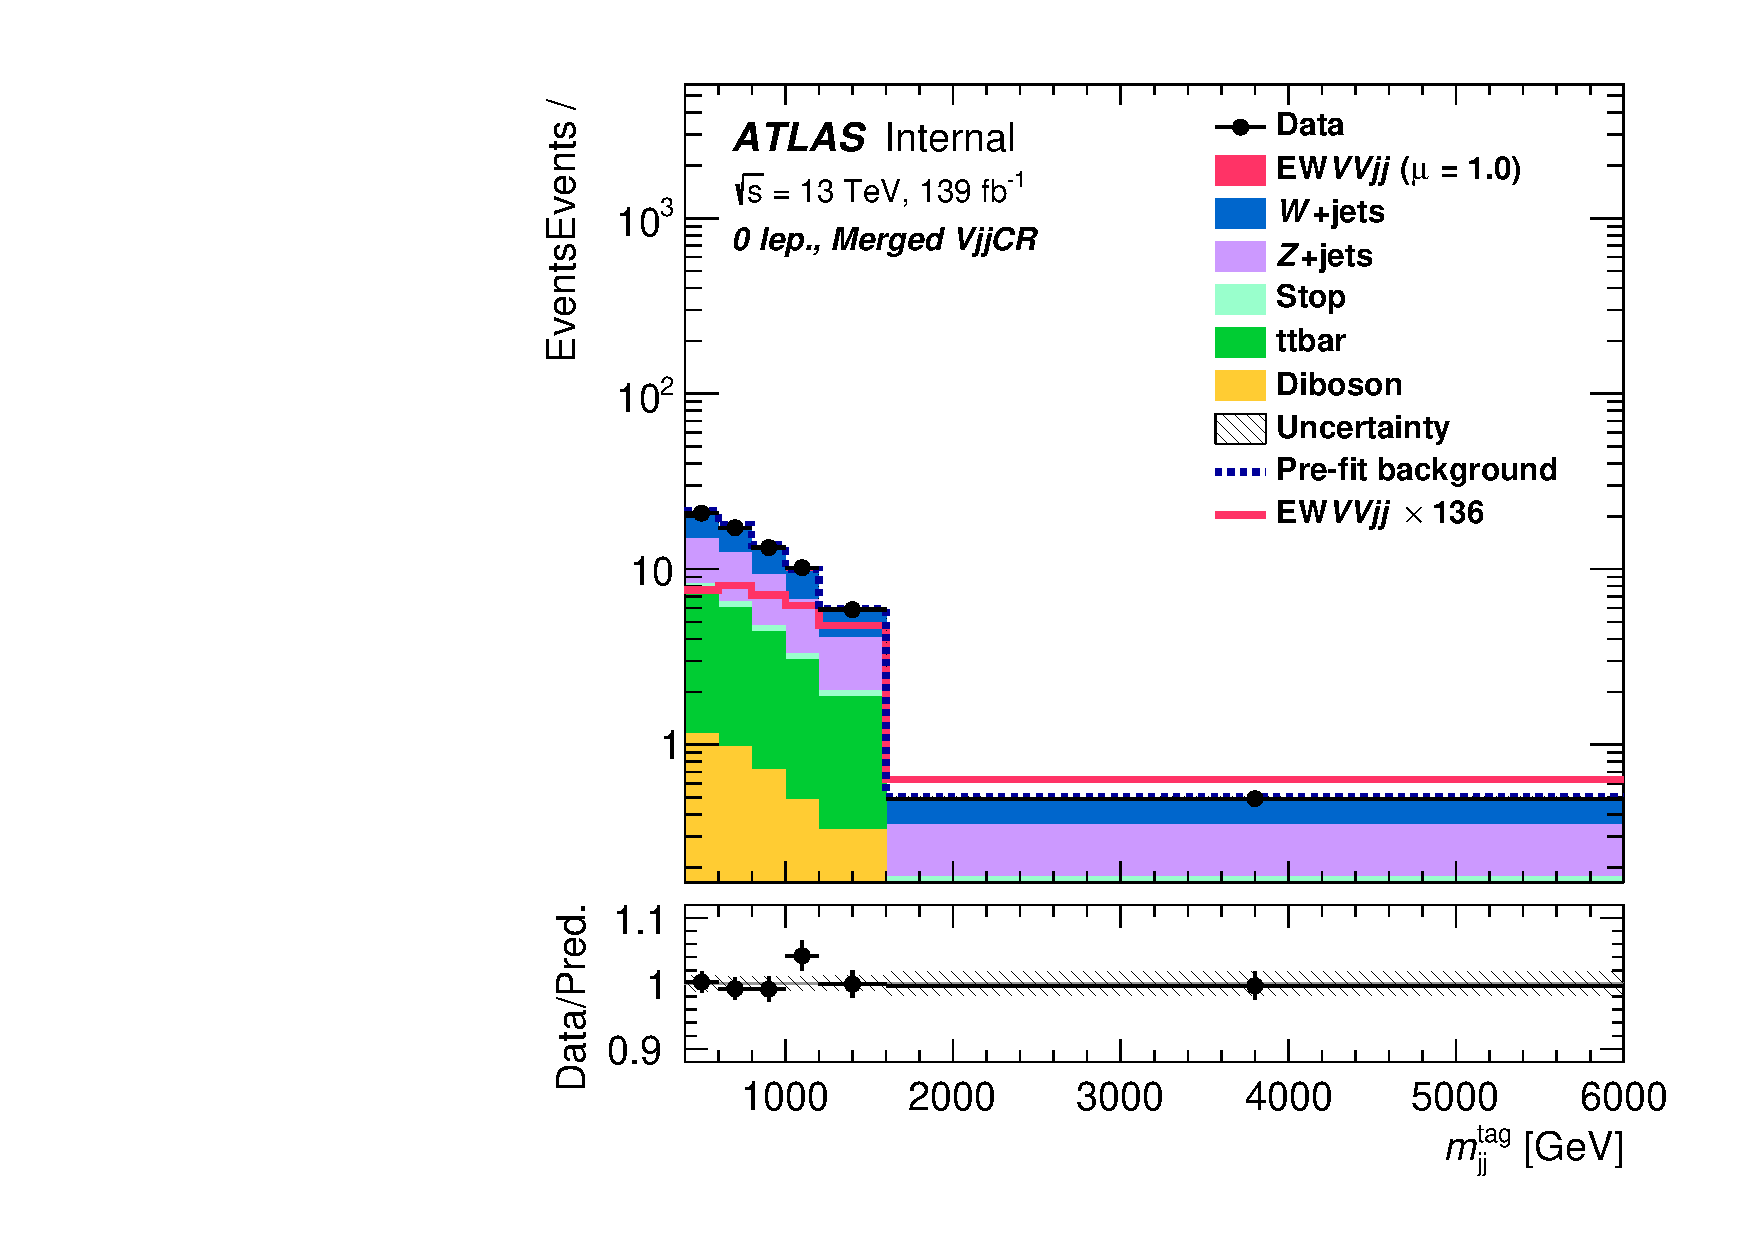
\includegraphics[width=0.45\textwidth]{figures/PostFit/Region_distMTagJets_DCRVjetMer_BMin0_J0_incJet1_L0_T0_incFat1_Y6051_incTag1_Fat1_GlobalFit_unconditionnal_mu1log}
    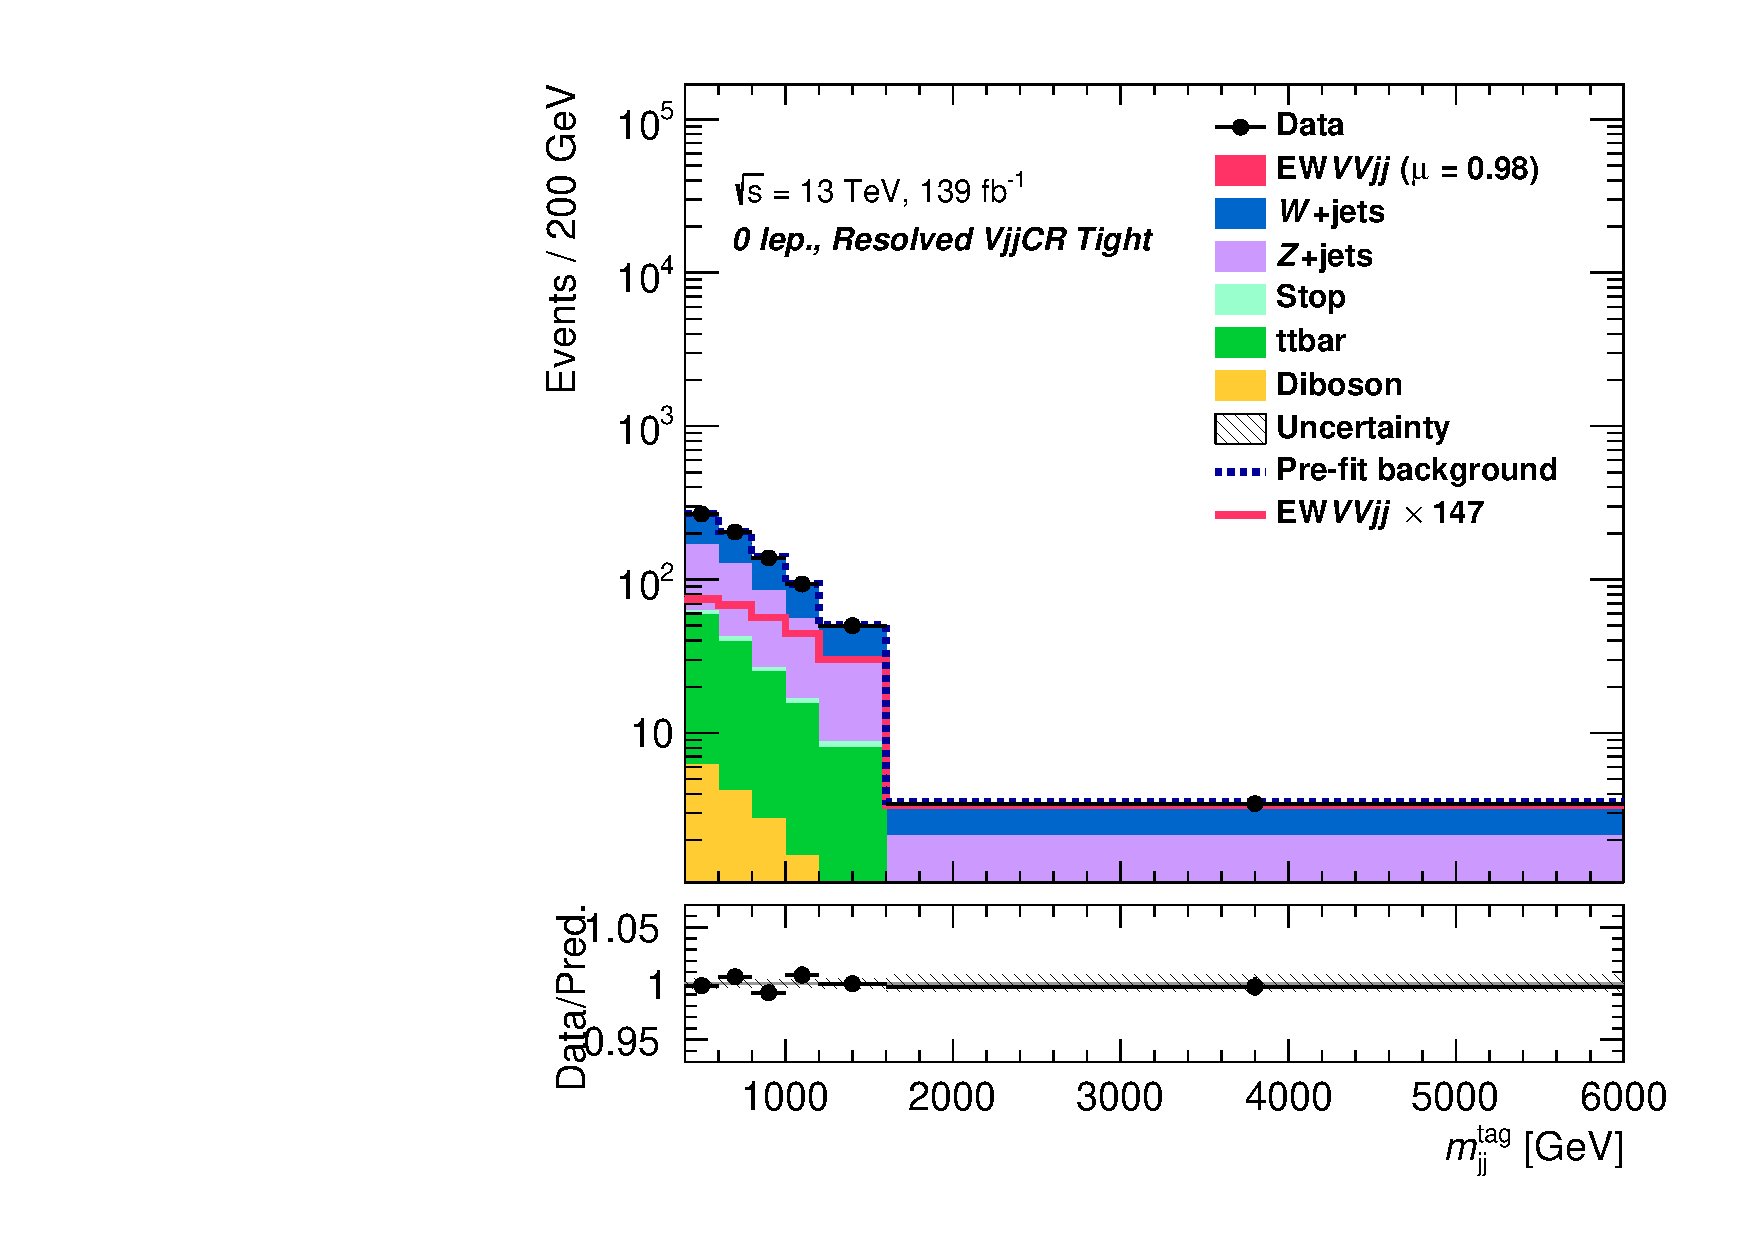
\includegraphics[width=0.45\textwidth]{figures/PostFit/Region_distMTagJets_DCRVjetFid_BMin0_T0_Y6051_incTag1_J2_L0_incJet1_GlobalFit_unconditionnal_mu1log}
    \\
    %1lep
    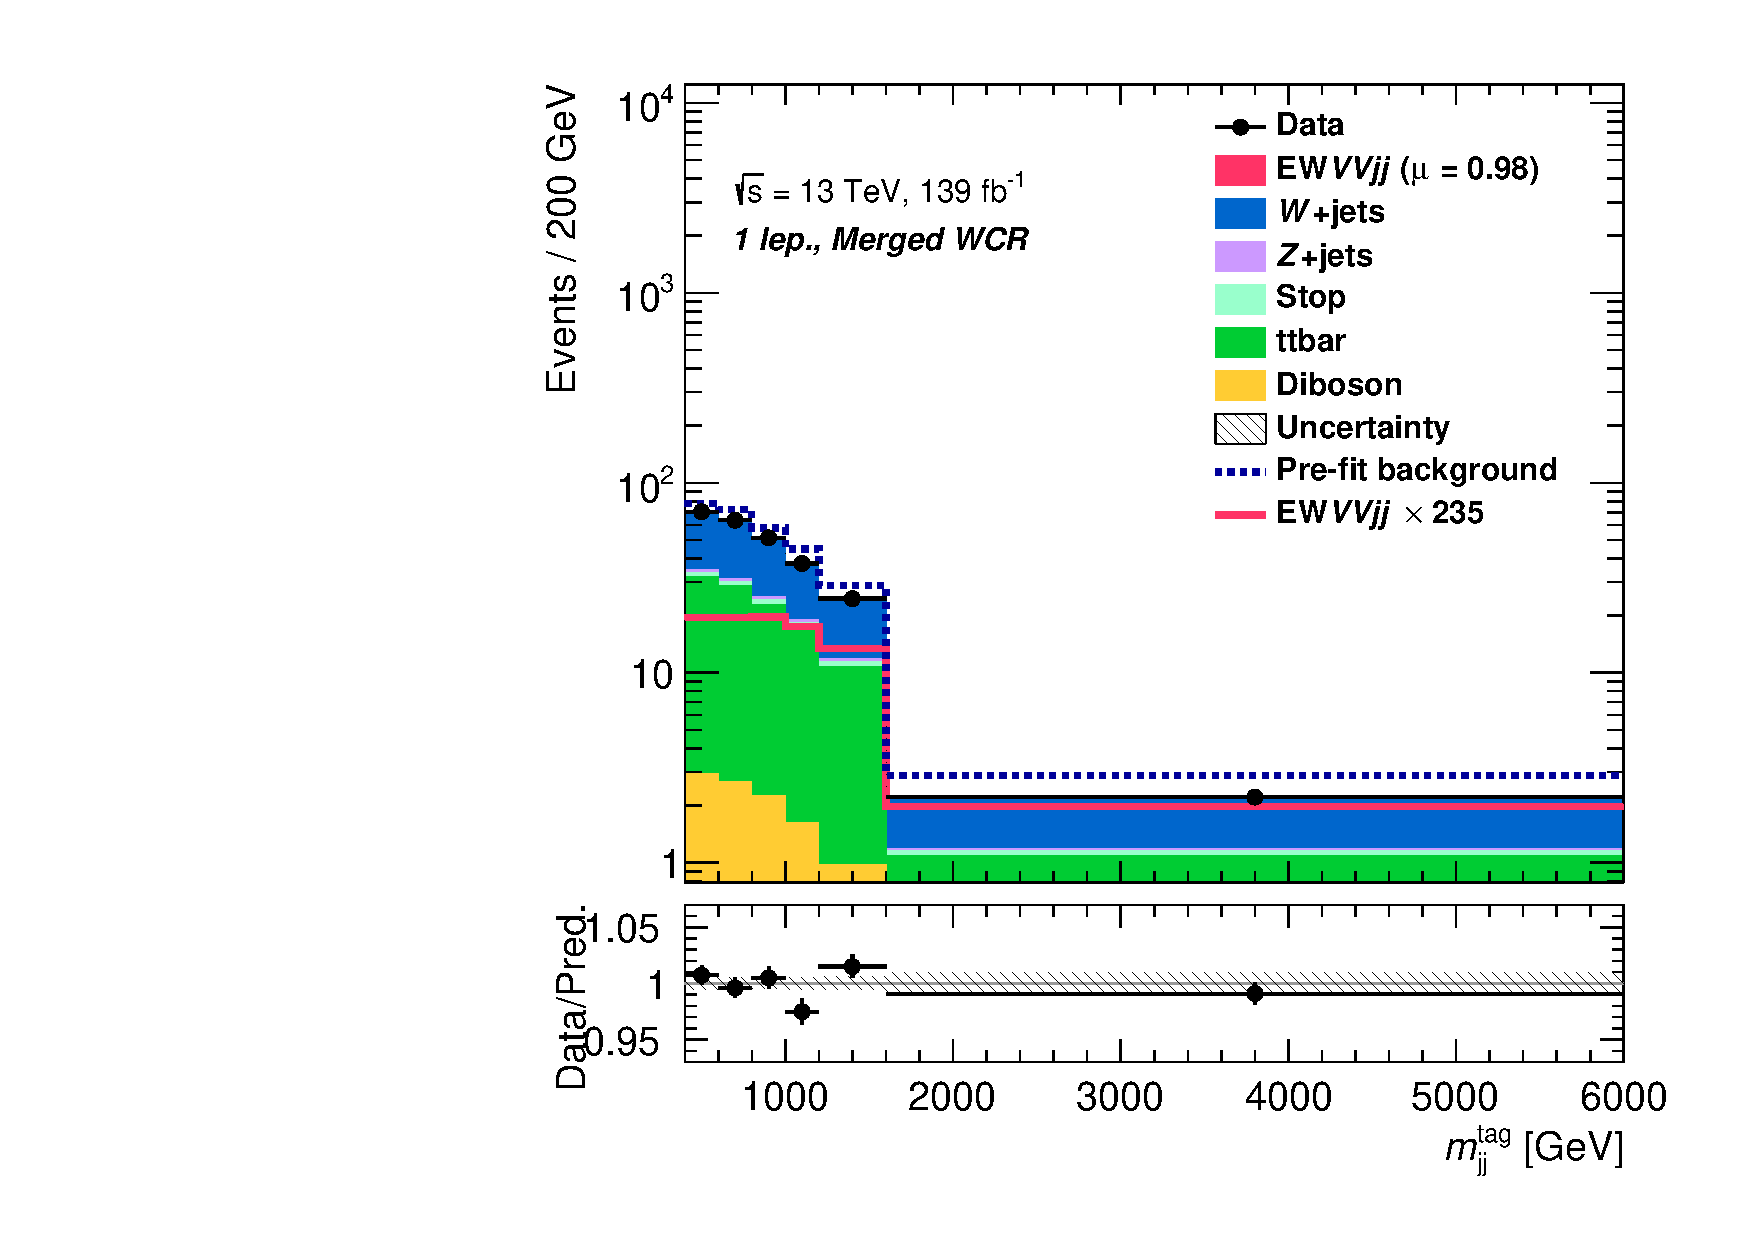
\includegraphics[width=0.45\textwidth]{figures/PostFit/Region_disttagMjj_DCRVjetMerged_BMin0_J0_incJet1_L1_T0_incFat1_Y6051_incTag1_Fat1_GlobalFit_unconditionnal_mu1log}
    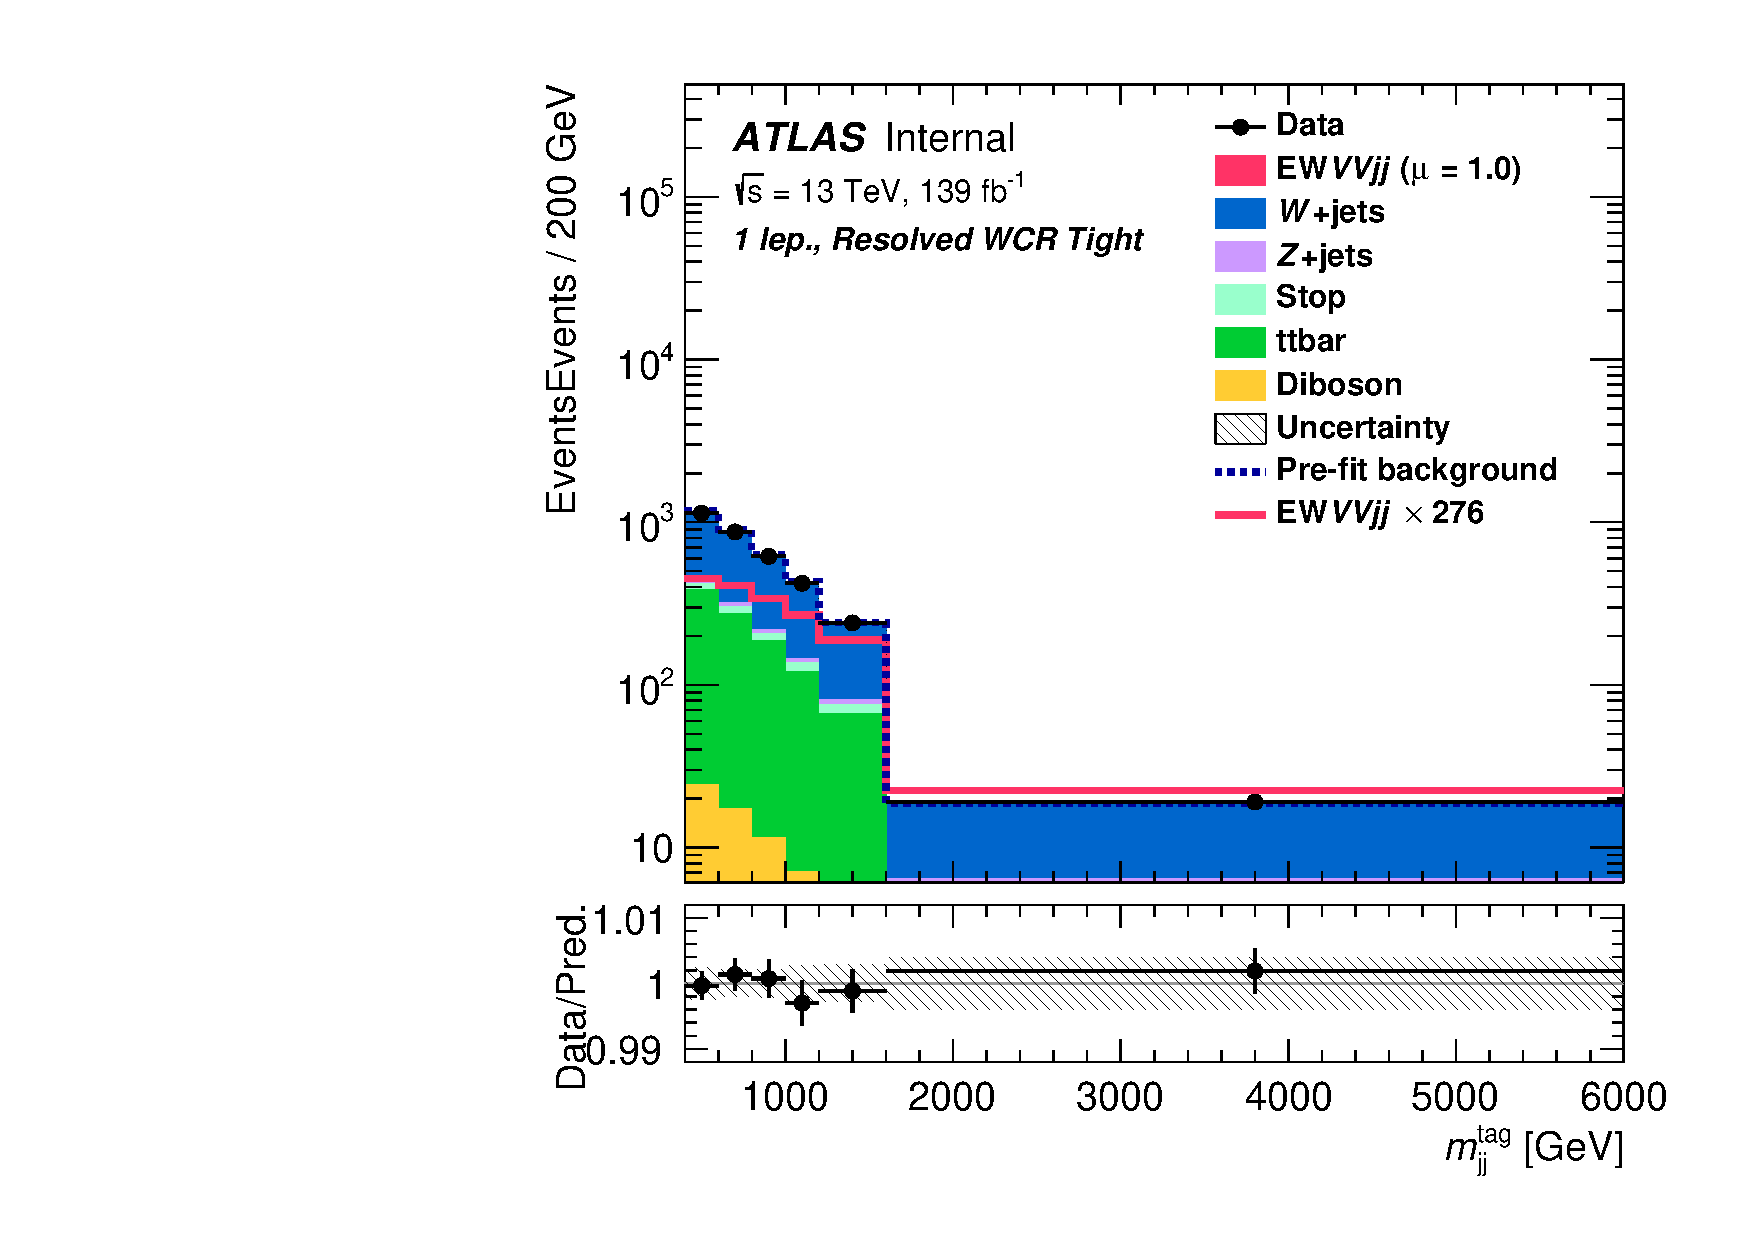
\includegraphics[width=0.45\textwidth]{figures/PostFit/Region_disttagMjj_DCRVjetTight_BMin0_T0_Y6051_incTag1_J2_L1_incJet1_GlobalFit_unconditionnal_mu1log}
    \\
    %2lep
     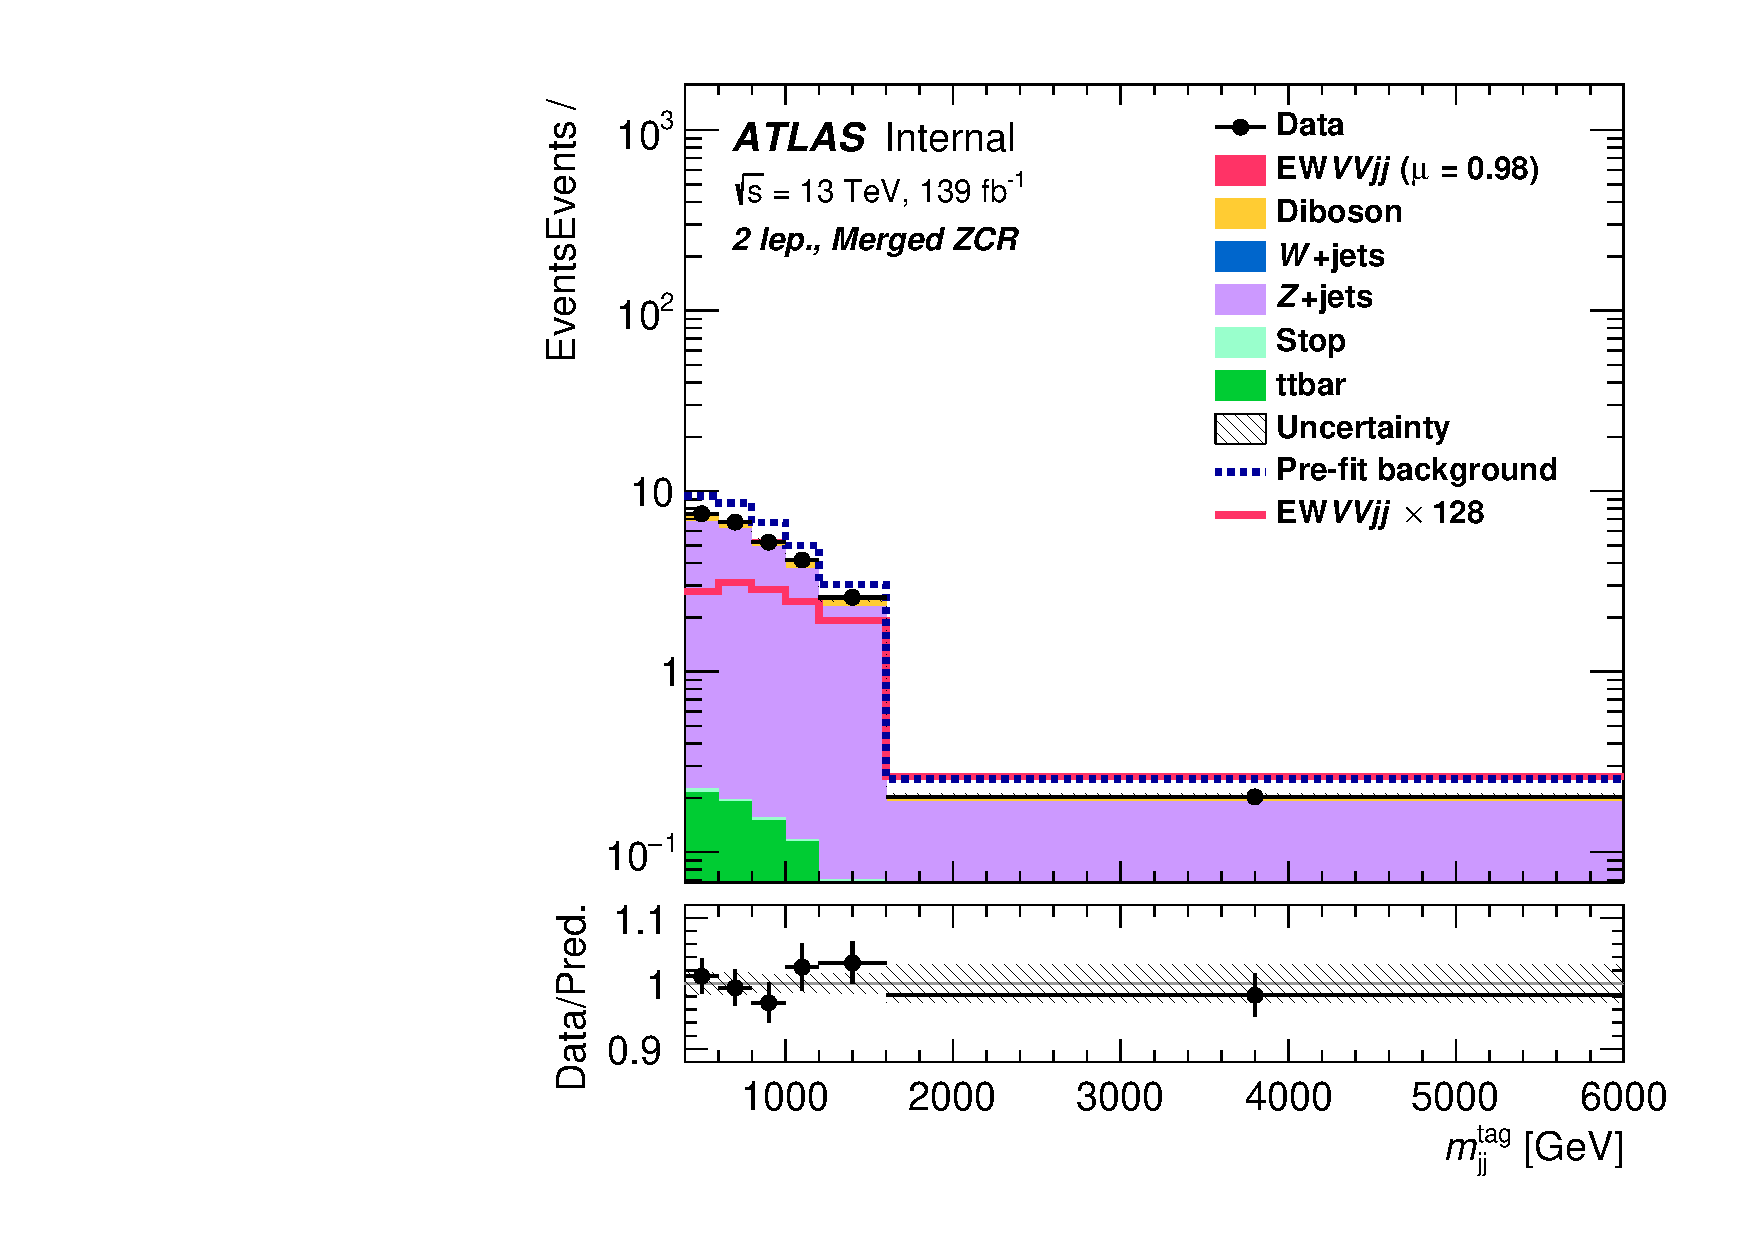
\includegraphics[width=0.45\textwidth]{figures/PostFit/Region_distMTagMerJets_DCRVjet_BMin0_J0_incJet1_L2_T0_incFat1_Y6051_incTag1_Fat1_GlobalFit_unconditionnal_mu1log}
      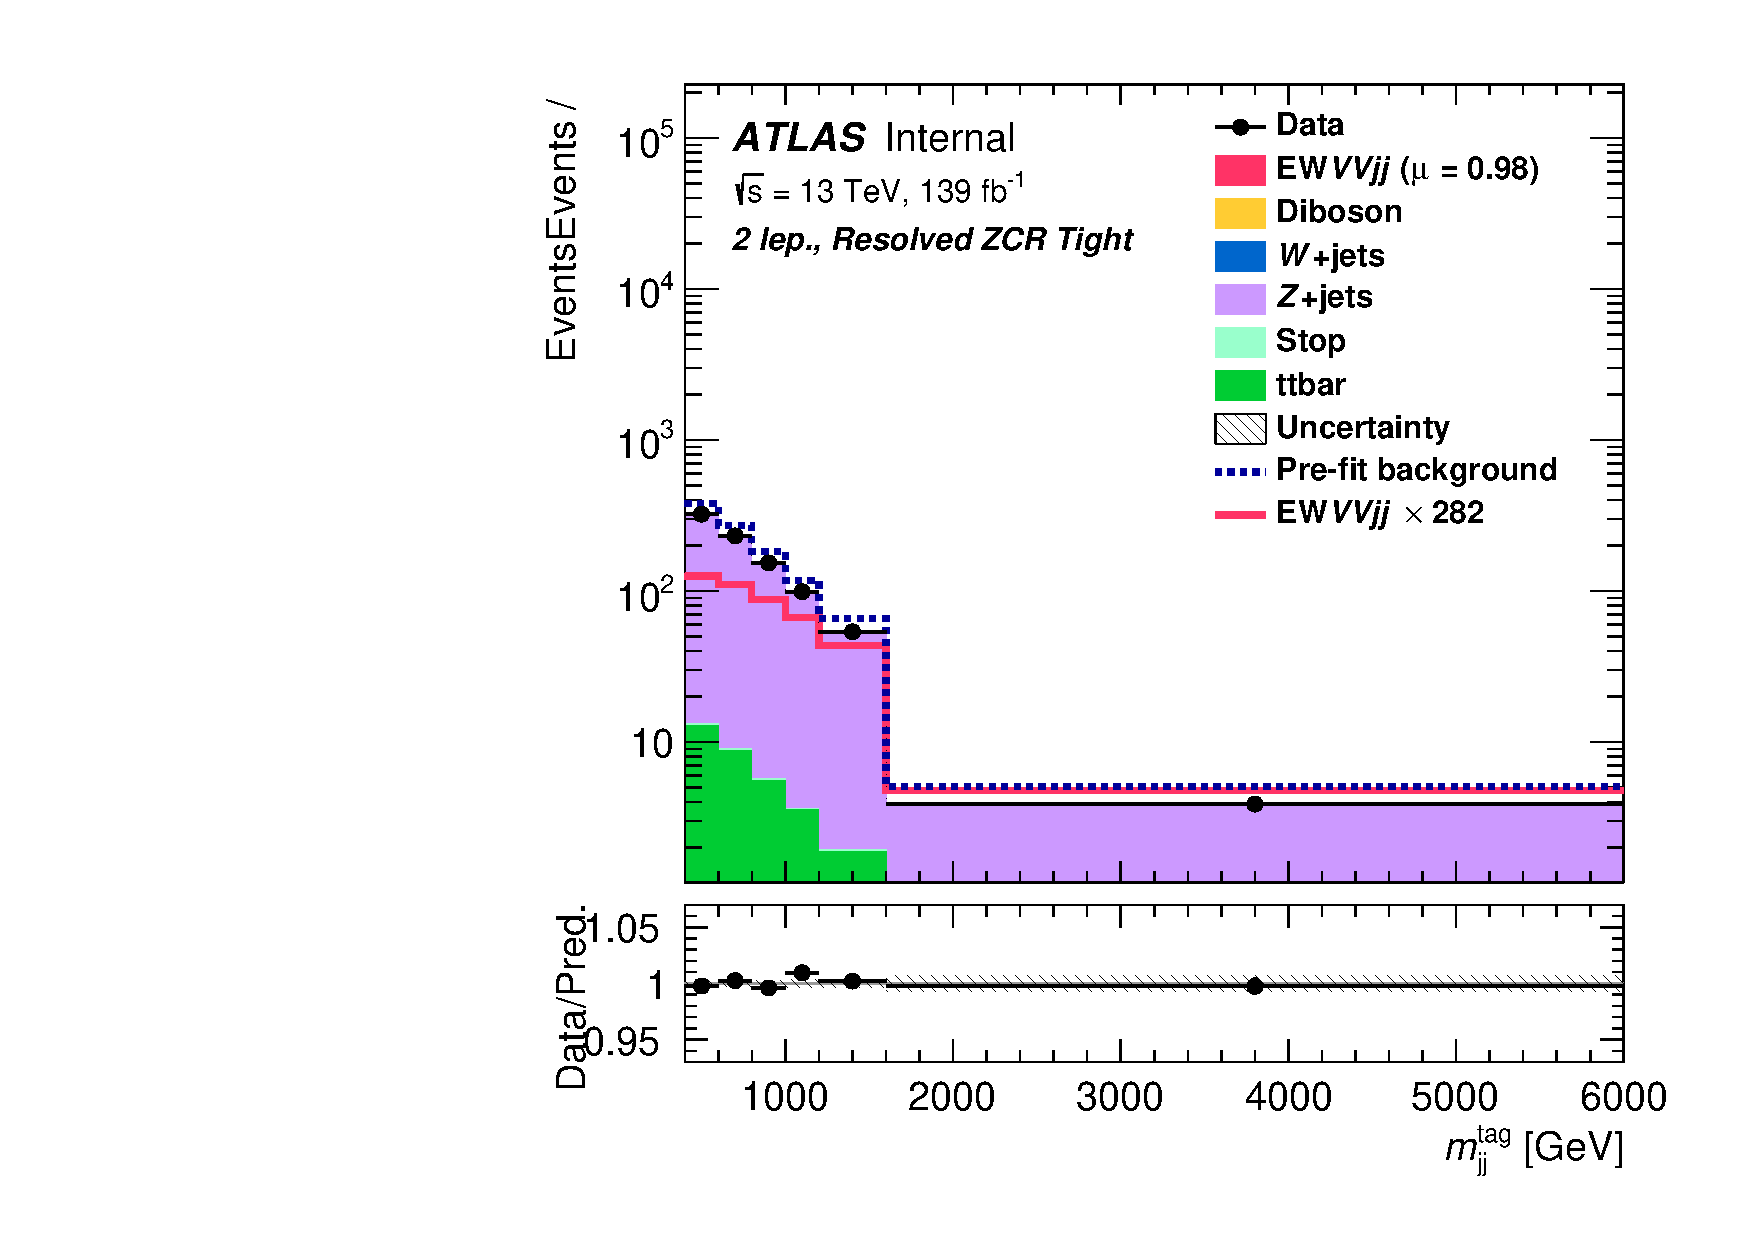
\includegraphics[width=0.45\textwidth]{figures/PostFit/Region_distMTagResJets_DCRVjetFid_BMin0_T0_Y6051_incTag1_J2_L2_incJet1_GlobalFit_unconditionnal_mu1log}
    \caption{Comparisons of the observed data and expected background distributions of $m^{tag}_{jj}$ in V+jets CRs in 0-lepton channel (1st line), 1-lepton channel (2nd line), and 2-lepton channel (3rd line). The EW VV+jj signal is filled on top of the fitted backgrounds, normalized to the signal yield extracted from the observed data ($\mu = 0.98$). The bottom panel show the ratio of the observed data to the post fit signal and background predictions.}
    \label{fig:postCR}
\end{figure}

\begin{figure}[]
    \centering
    %1lep
    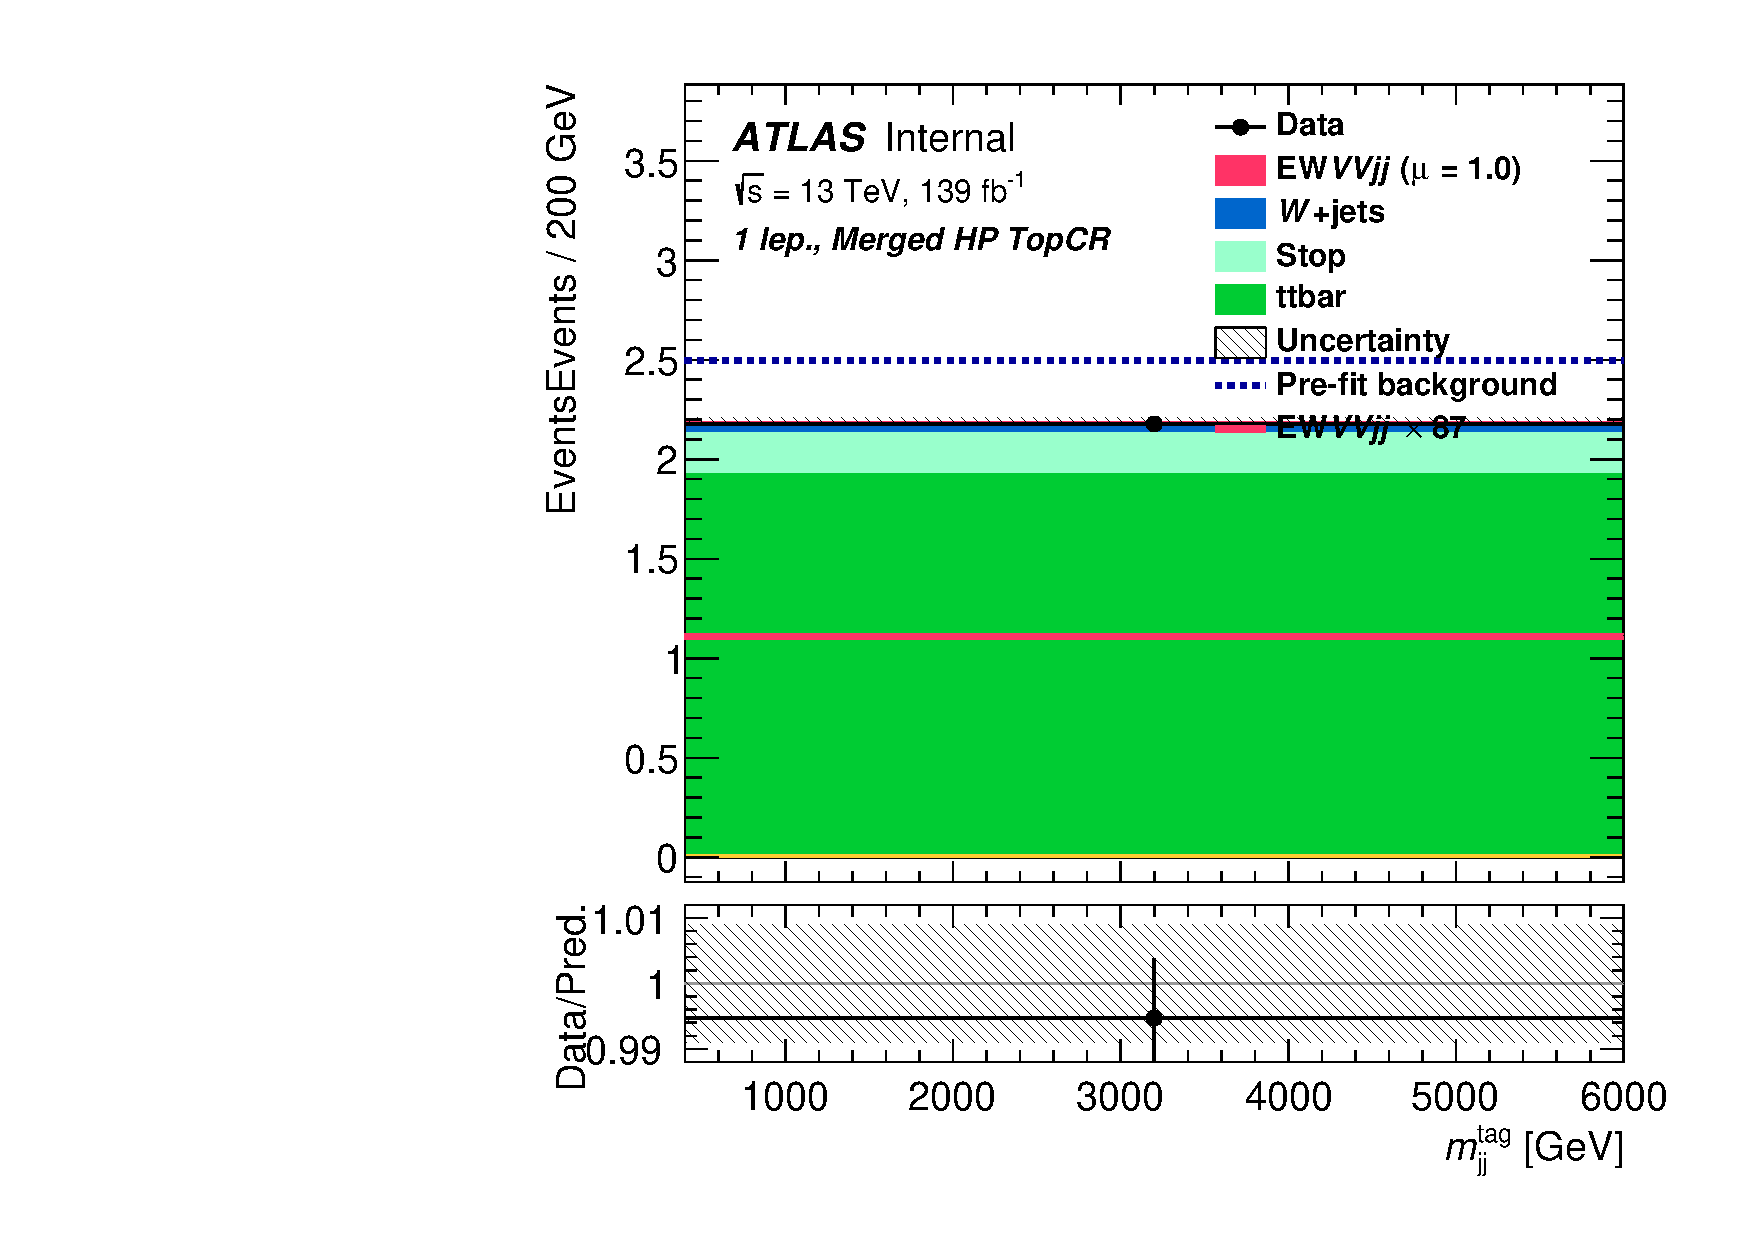
\includegraphics[width=0.45\textwidth]{figures/PostFit/Region_disttagMjj_DCRTopHP_BMin0_J0_incJet1_L1_T0_incFat1_Y6051_incTag1_Fat1_GlobalFit_unconditionnal_mu1}
    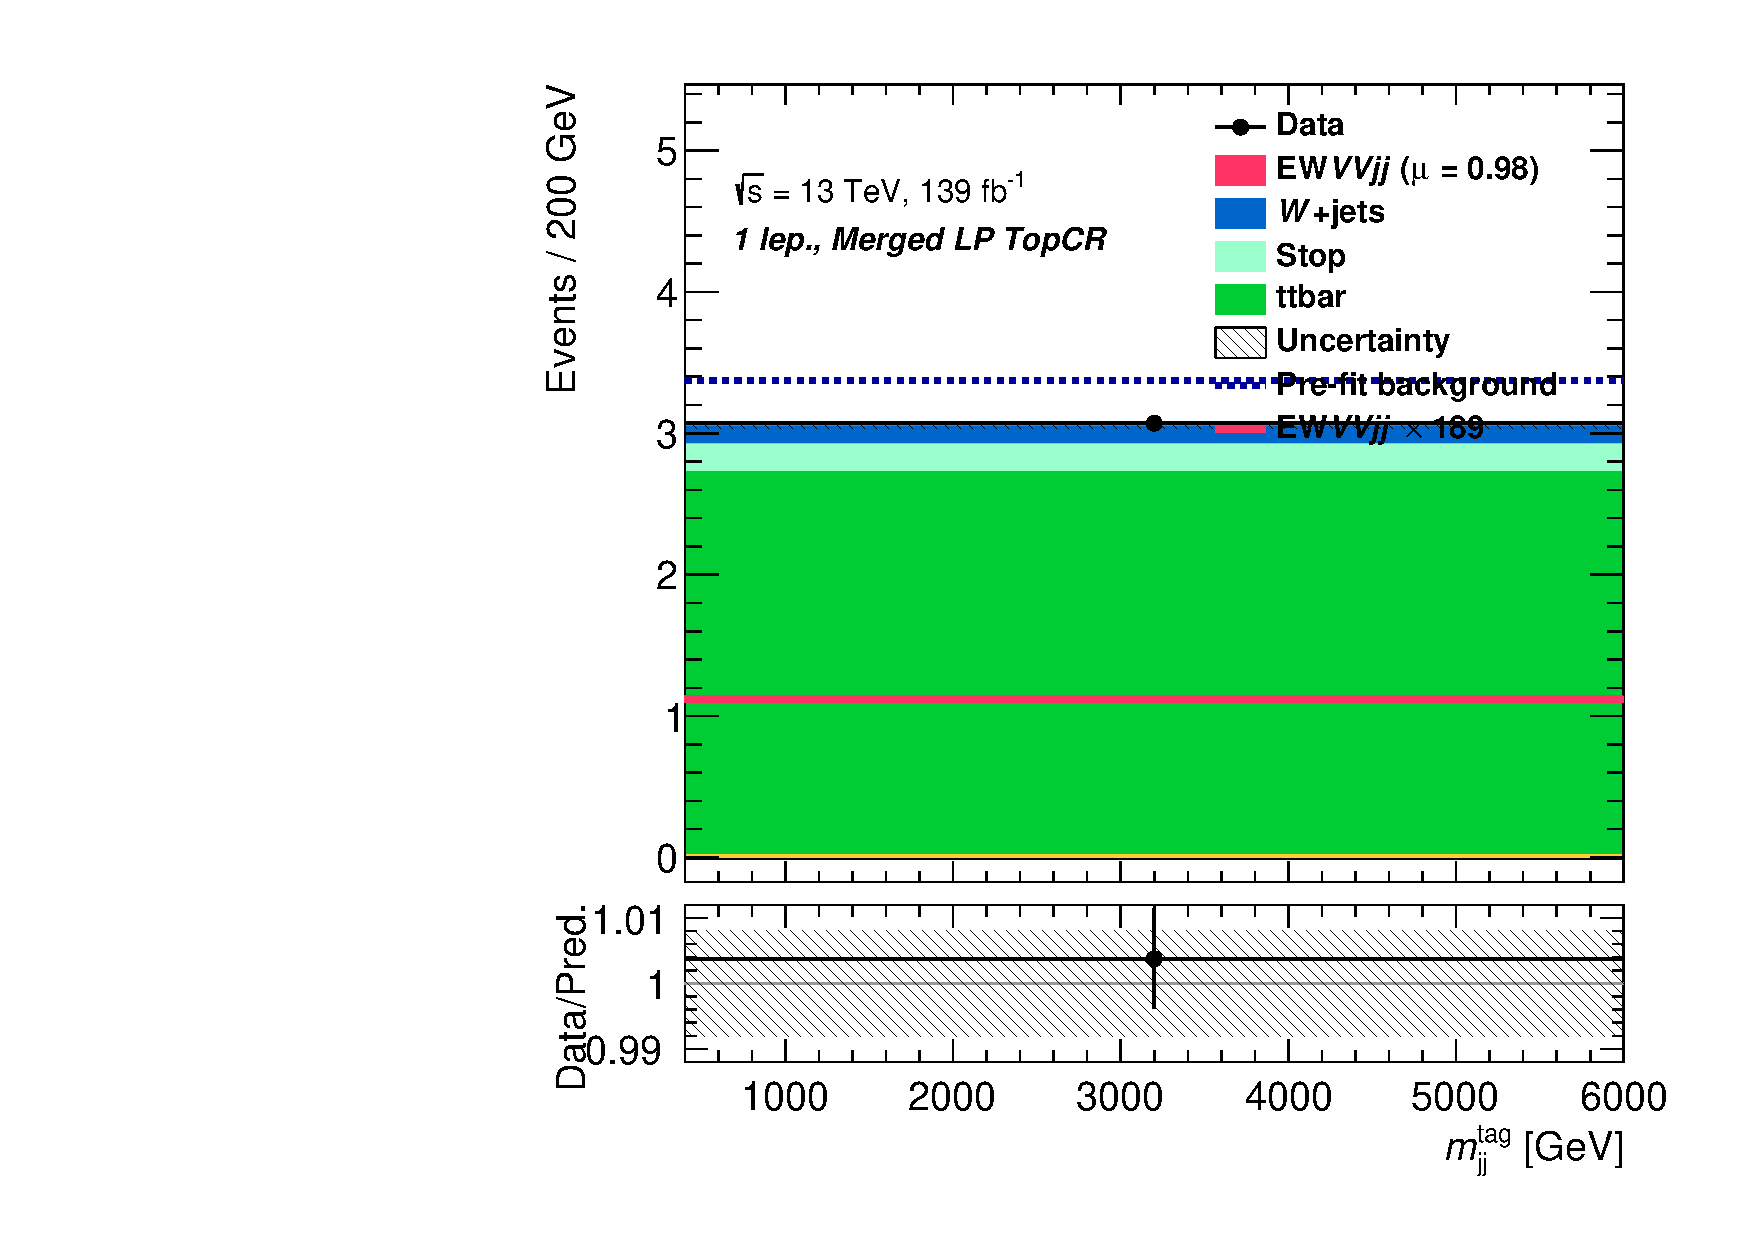
\includegraphics[width=0.45\textwidth]{figures/PostFit/Region_disttagMjj_DCRTopLP_BMin0_J0_incJet1_L1_T0_incFat1_Y6051_incTag1_Fat1_GlobalFit_unconditionnal_mu1}
    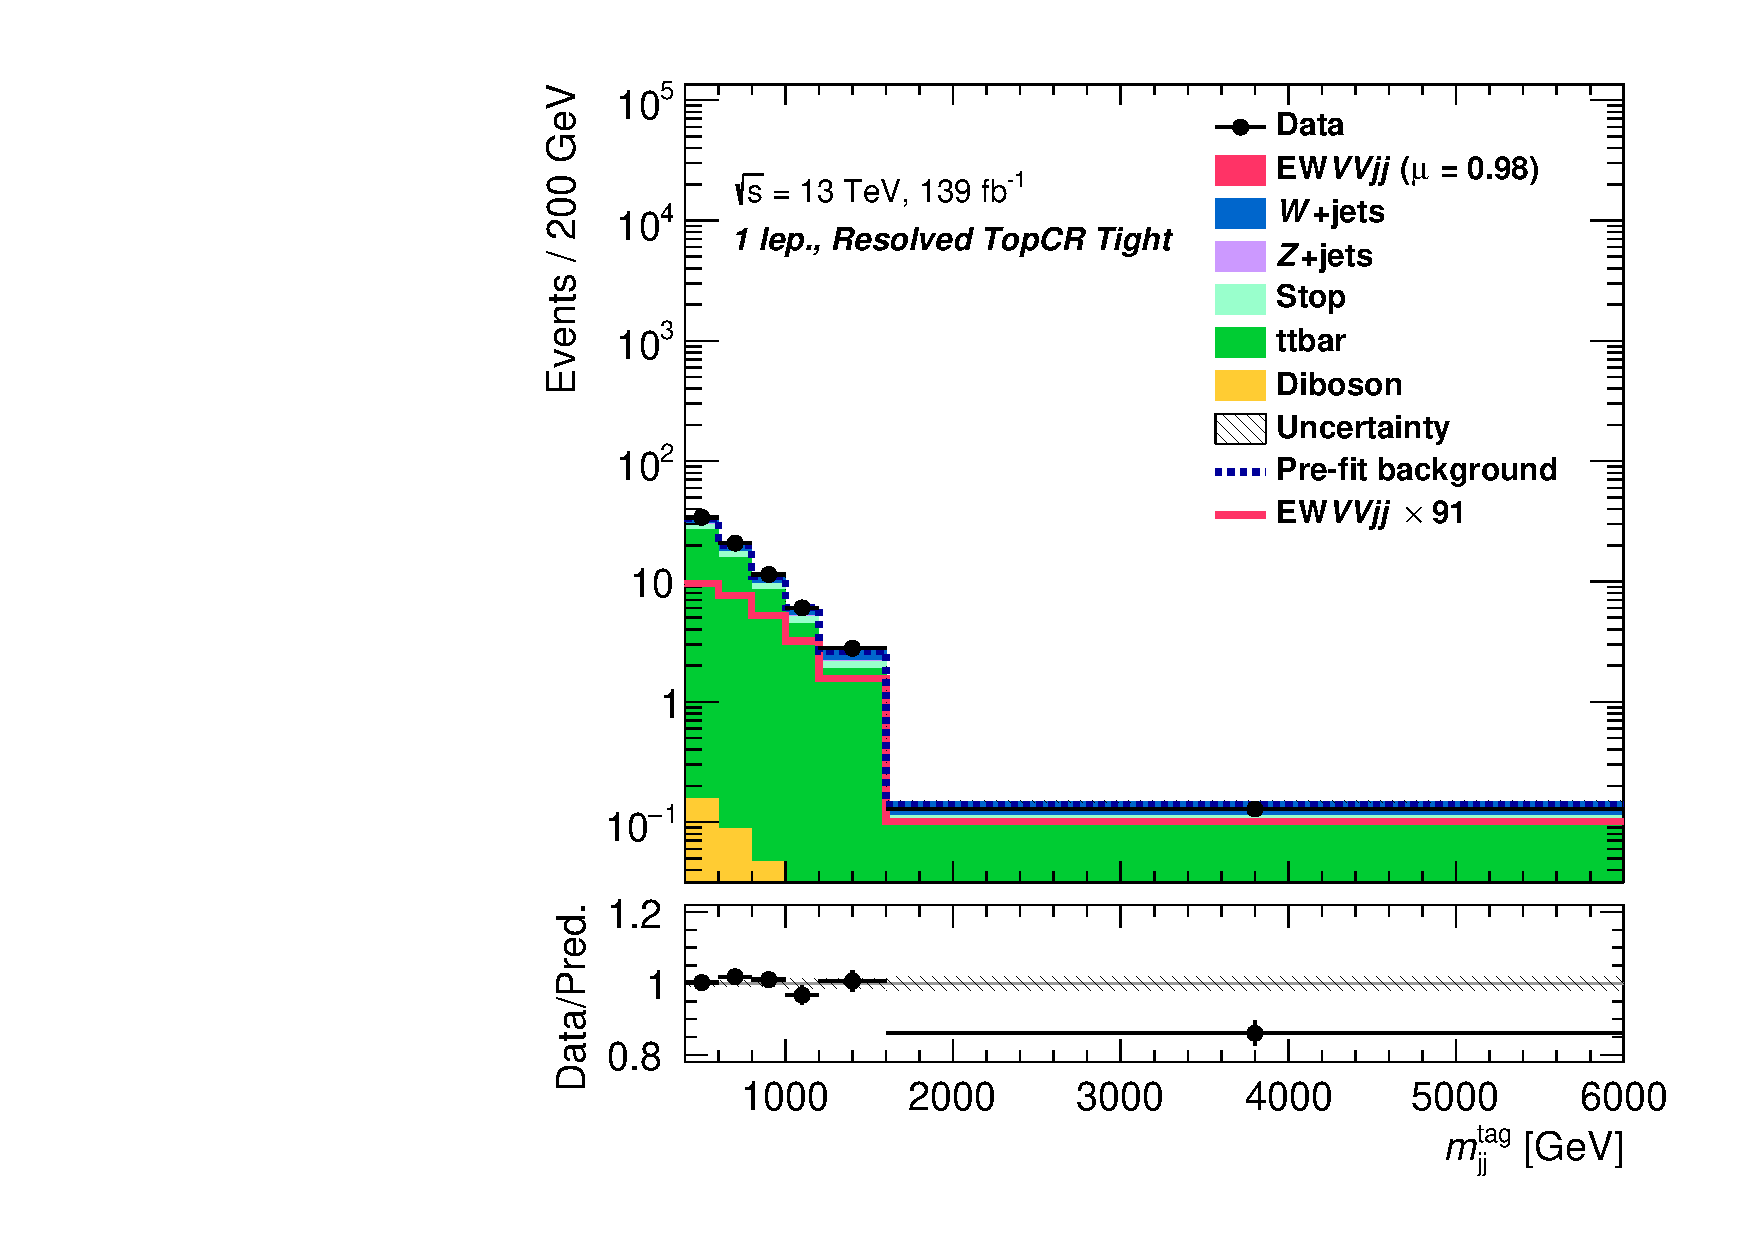
\includegraphics[width=0.45\textwidth]{figures/PostFit/Region_disttagMjj_DCRTopTight_BMin0_T0_Y6051_incTag1_J2_L1_incJet1_GlobalFit_unconditionnal_mu1log} 
    \caption{Comparisons of the observed data and expected background distributions of $m^{tag}_{jj}$ in Top CRs in 1-lepton channel.  The EW VV+jj signal is filled on top of the fitted backgrounds, normalized to the signal yield extracted from the observed data ($\mu = 0.98$). The bottom panel shows the ratio of the observed data to the post fit signal and background predictions.}
    \label{fig:postCRTop}
\end{figure}

%\noindent\textbf{\sf{RNN score distributions at SRs after fitting}}\\
\subsection{RNN score distributions at SRs after fitting}
The RNN score distributions in each SRs after fitting are shown in figure~\ref{fig:postSR0lep}, \ref{fig:postSR1lep}, \ref{fig:postSR2lep}.
In the low-RNN score bins, where the events are dominated by the background samples, the predicted MCs nicely reproduce the observed data in each region and channel. In the right-most bins which include signal contribution, a little overshoot can be seen, especially for 0-lepton Merged HP region and Resolved region. In most regions, the background yields are decreased in low-RNN bins after fitting, while increased in high-RNN bins, which can be the effect of the NPs that change RNN score shapes, mainly the modeling uncertainty of the V+jets sample.

%signal region
\begin{figure}[]
    \centering
    %0lep
    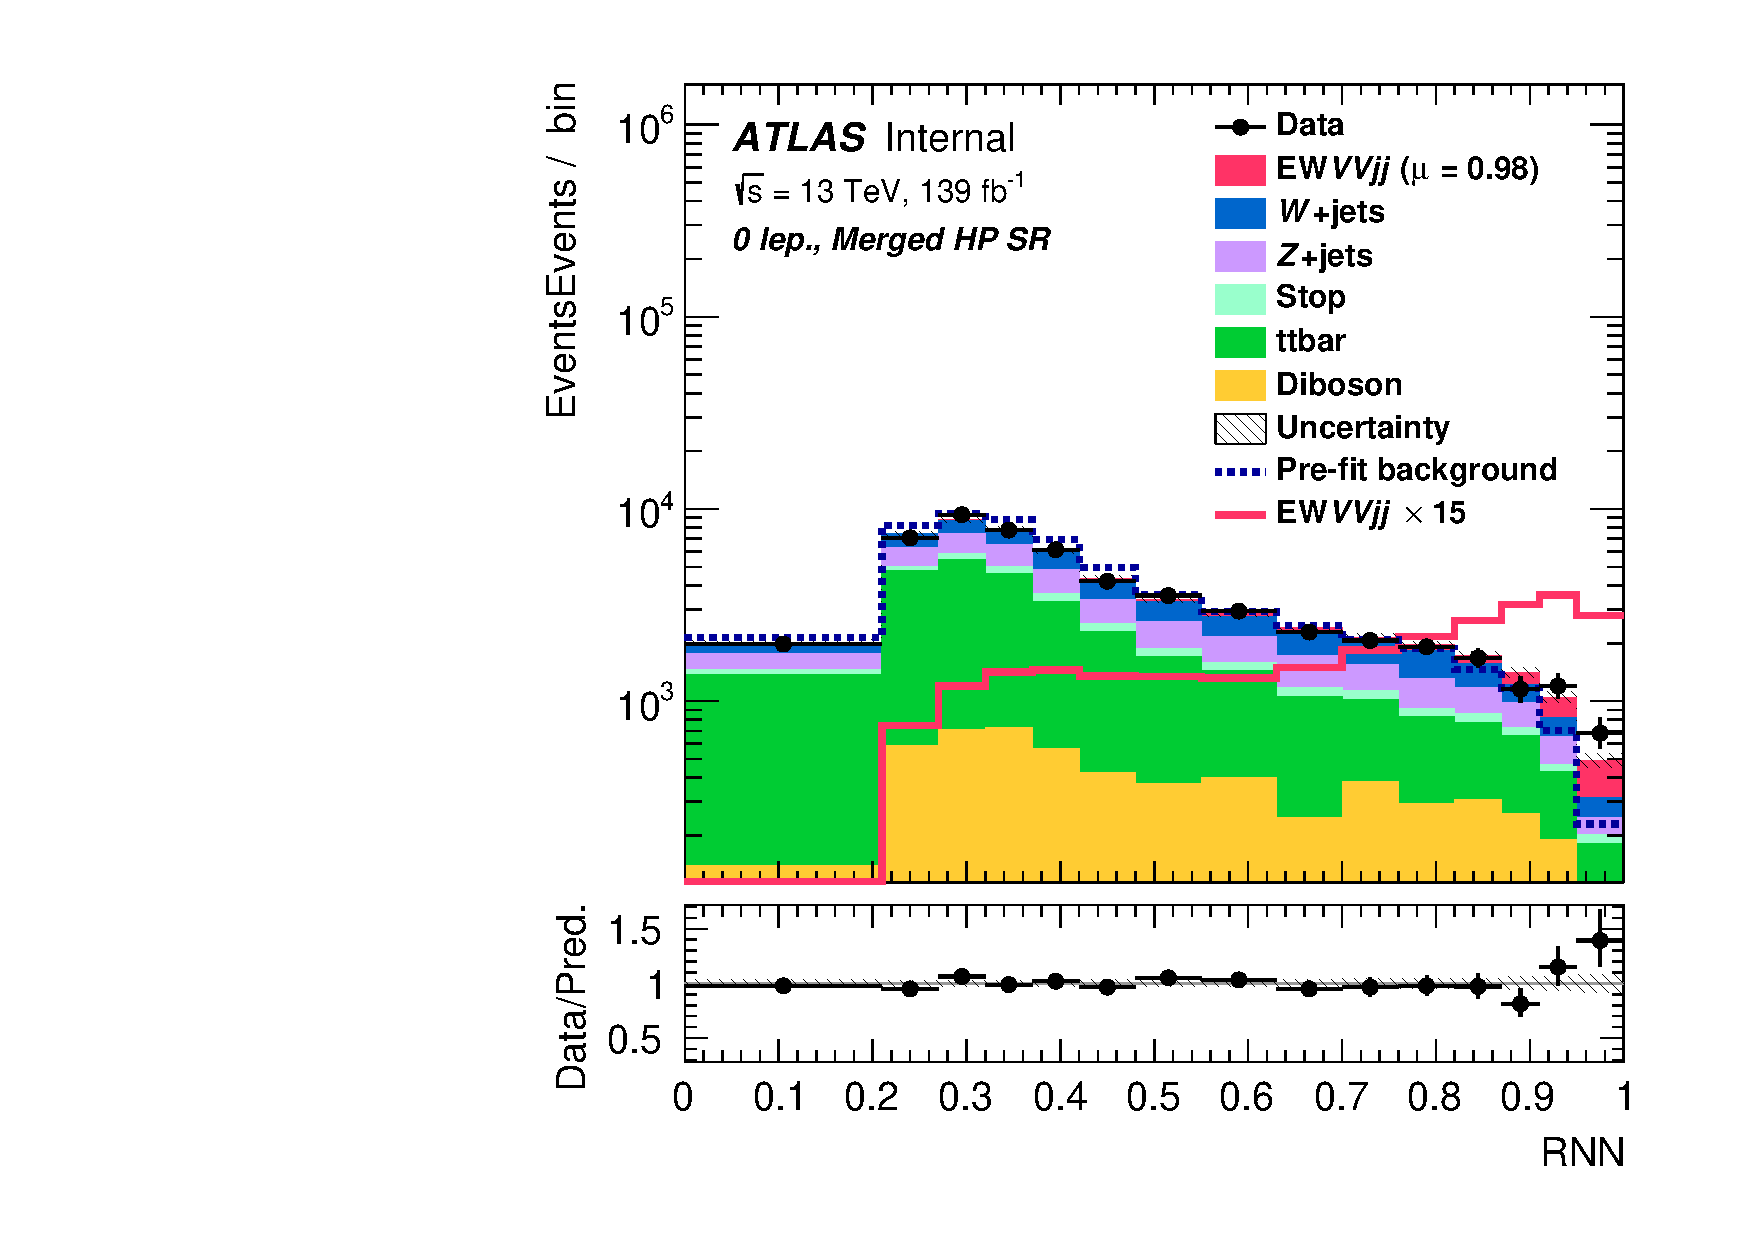
\includegraphics[width=0.45\textwidth]{figures/PostFit/Region_distRNN_DSRVBSHP_BMin0_J0_incJet1_L0_T0_incFat1_Y6051_incTag1_Fat1_GlobalFit_unconditionnal_mu1log}
    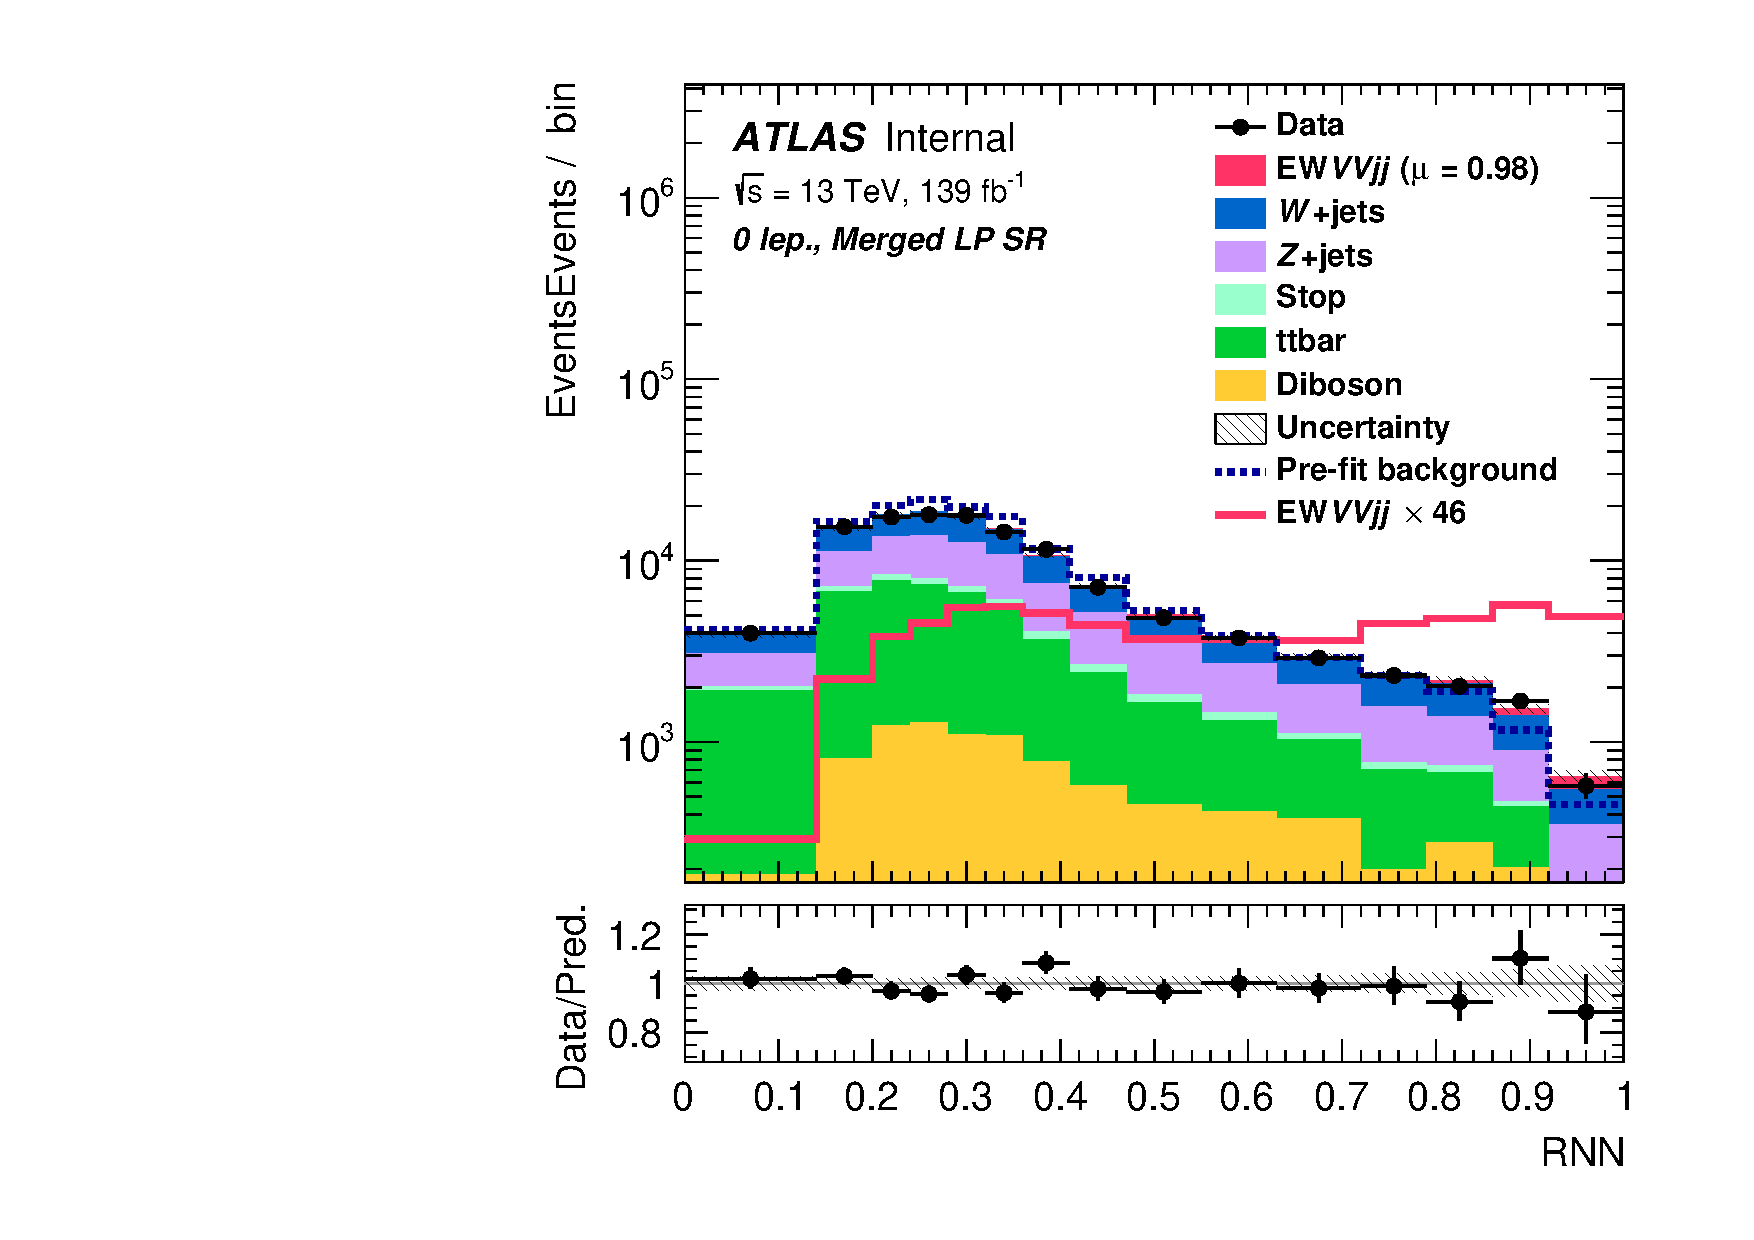
\includegraphics[width=0.45\textwidth]{figures/PostFit/Region_distRNN_DSRVBSLP_BMin0_J0_incJet1_L0_T0_incFat1_Y6051_incTag1_Fat1_GlobalFit_unconditionnal_mu1log}
    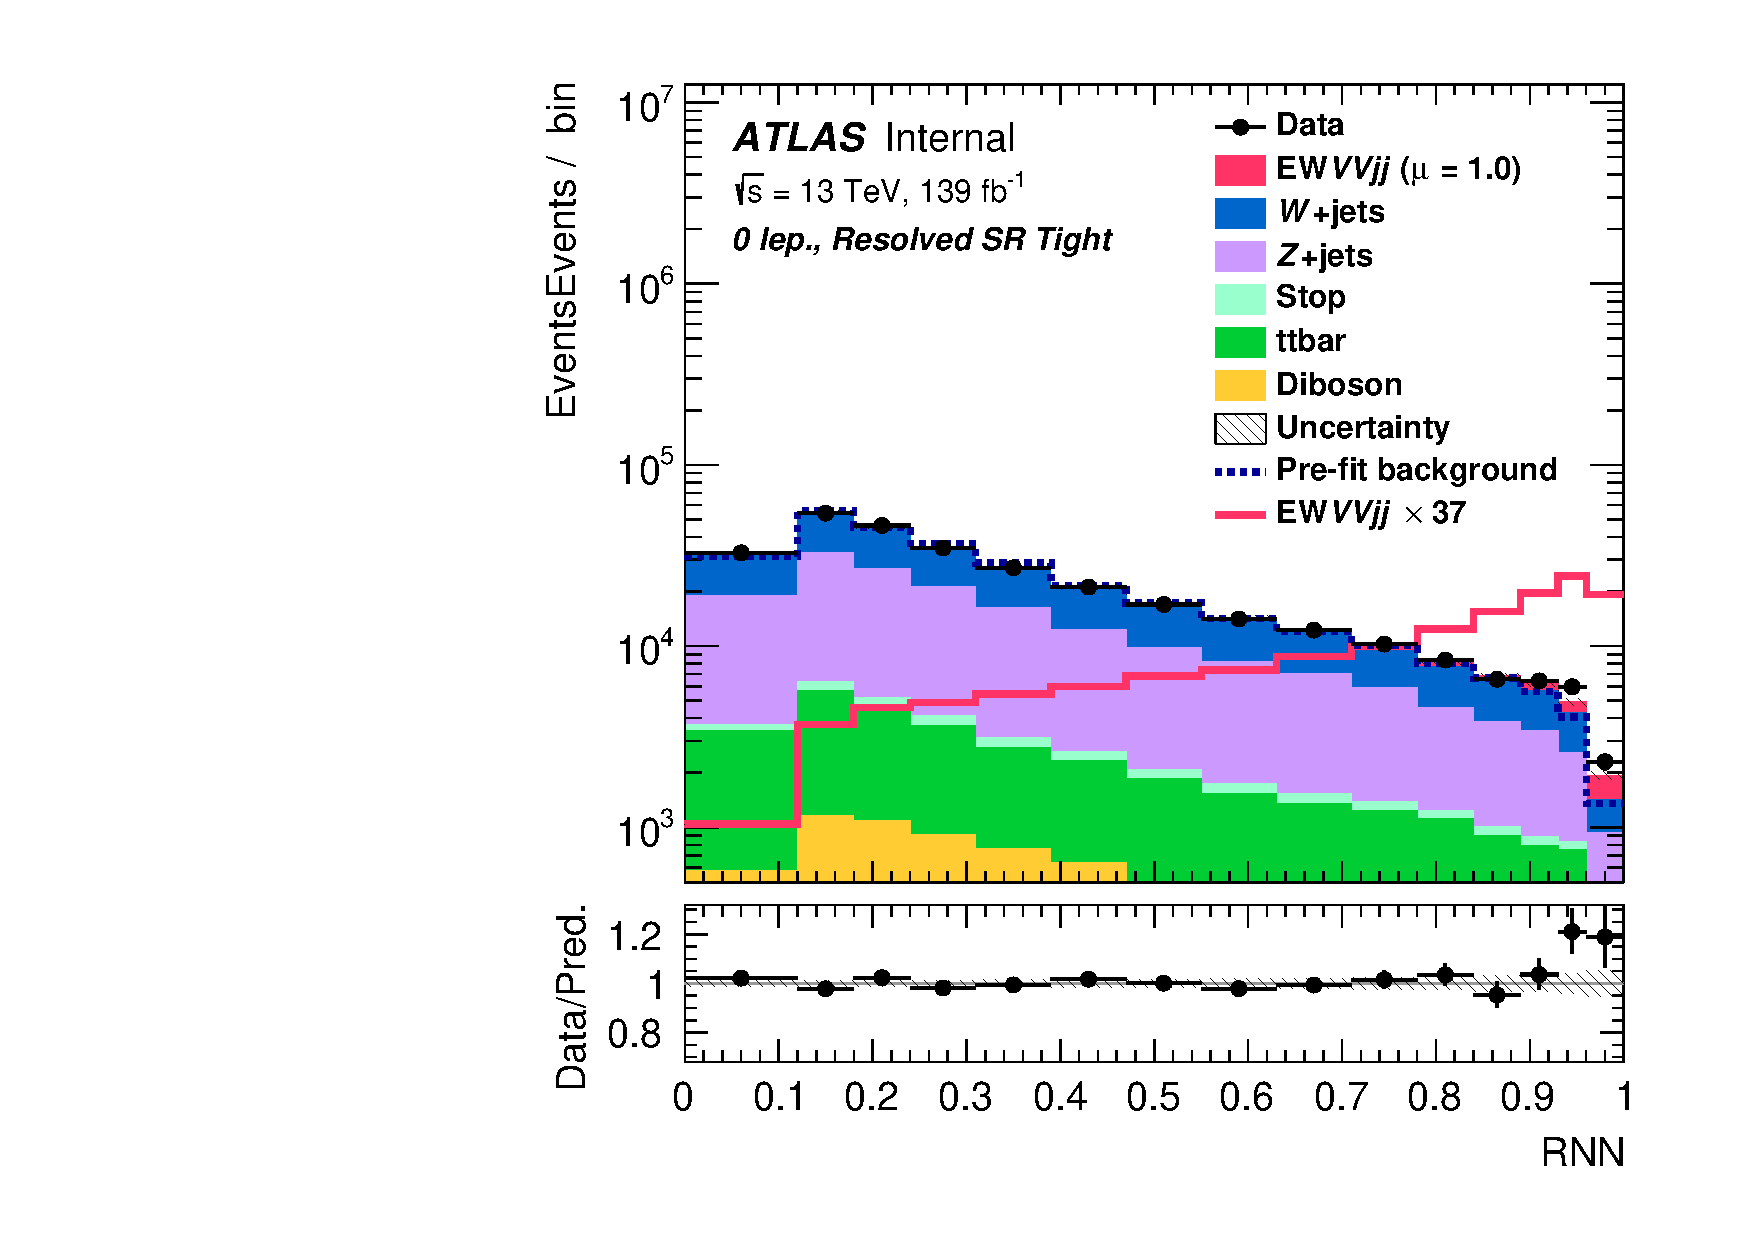
\includegraphics[width=0.45\textwidth]{figures/PostFit/Region_distRNN_DSRVBSFid_BMin0_T0_Y6051_incTag1_J2_L0_incJet1_GlobalFit_unconditionnal_mu1log}
      \caption{Comparisons of the observed data and expected background distributions of RNN score in 0-lepton channel signal regions. The EW VV+jj signal is filled on top of the fitted backgrounds, normalized to the signal yield extracted from the observed data ($\mu = 0.98$). The bottom panel shows the ratio of the observed data to the post fit signal and background predictions.}
      \label{fig:postSR0lep}
\end{figure}
\begin{figure}[]
    \centering
    %1lep
    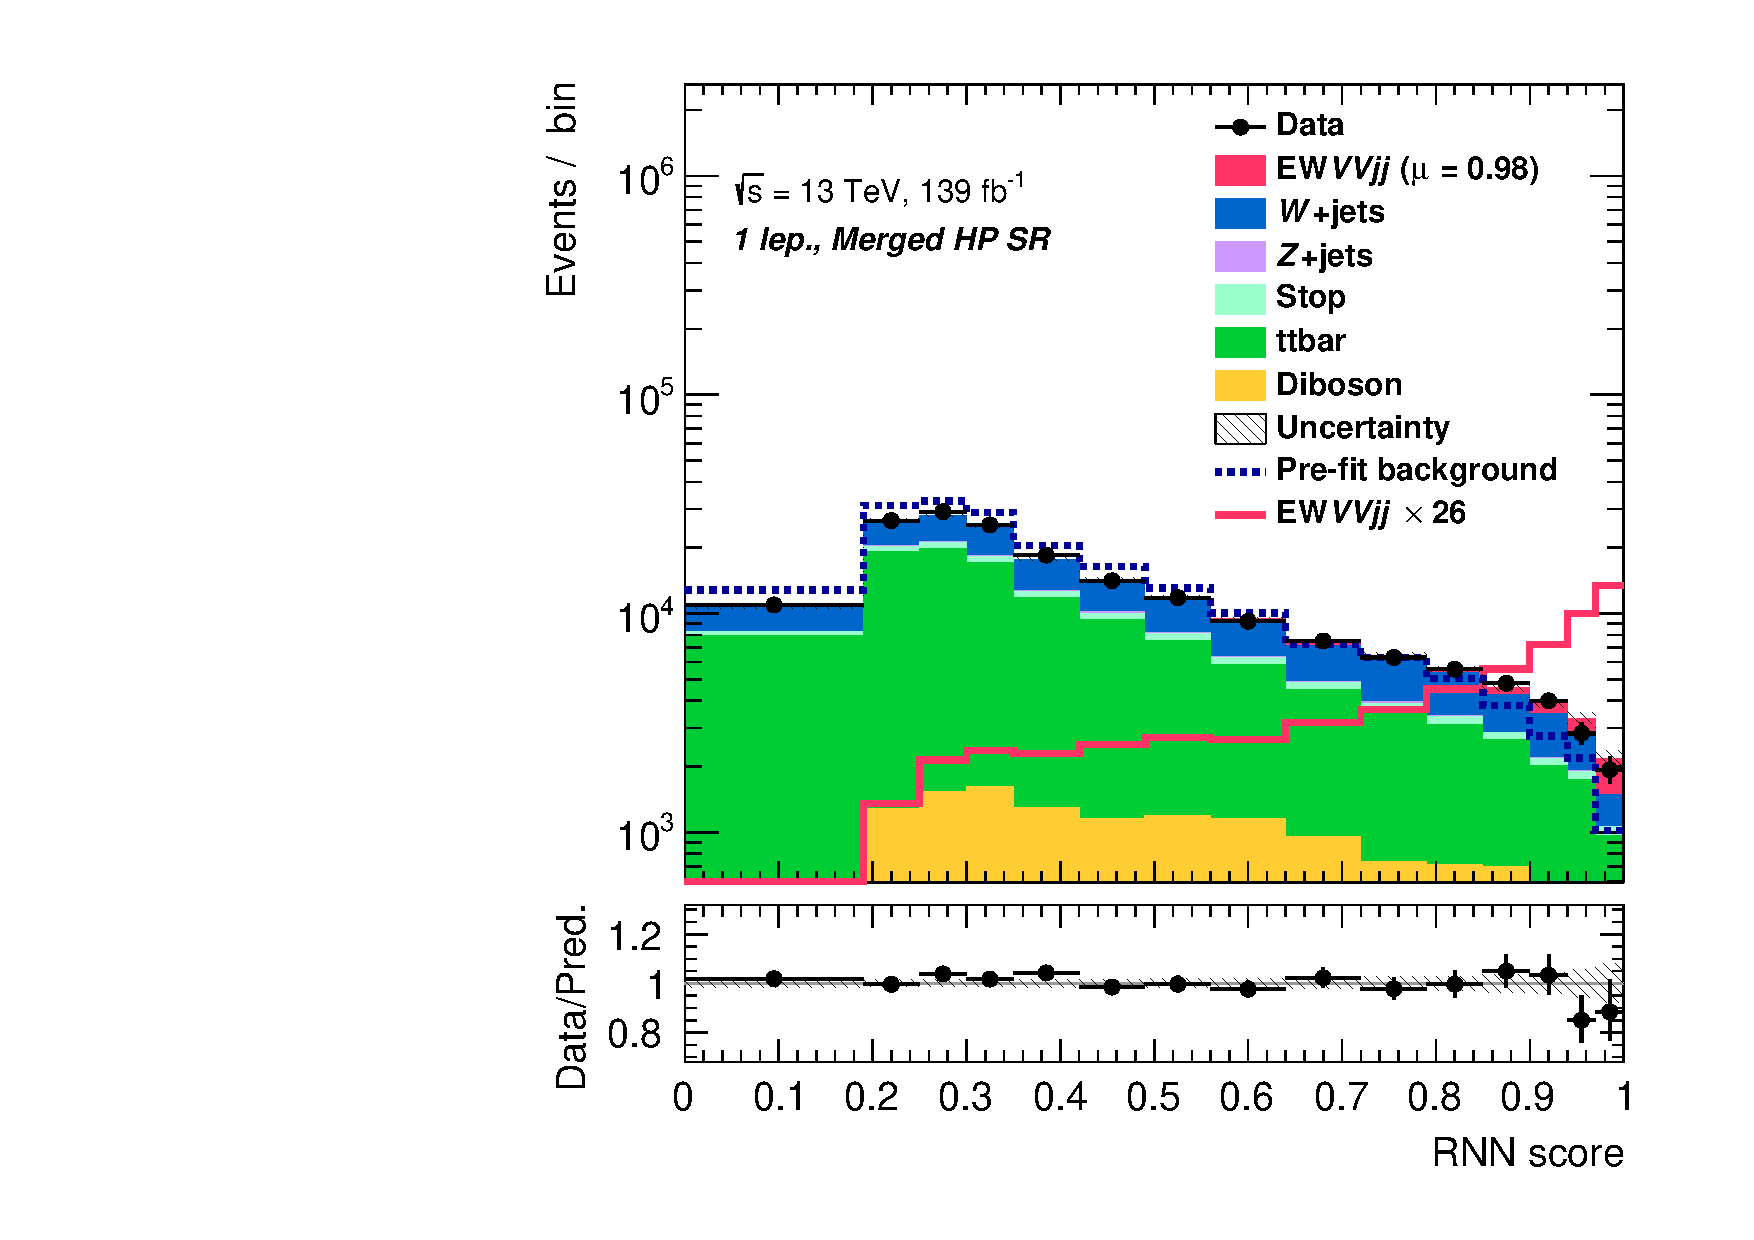
\includegraphics[width=0.45\textwidth]{figures/PostFit/Region_distRNN_DSRVBSHP_BMin0_J0_incJet1_L1_T0_incFat1_Y6051_incTag1_Fat1_GlobalFit_unconditionnal_mu1log}
    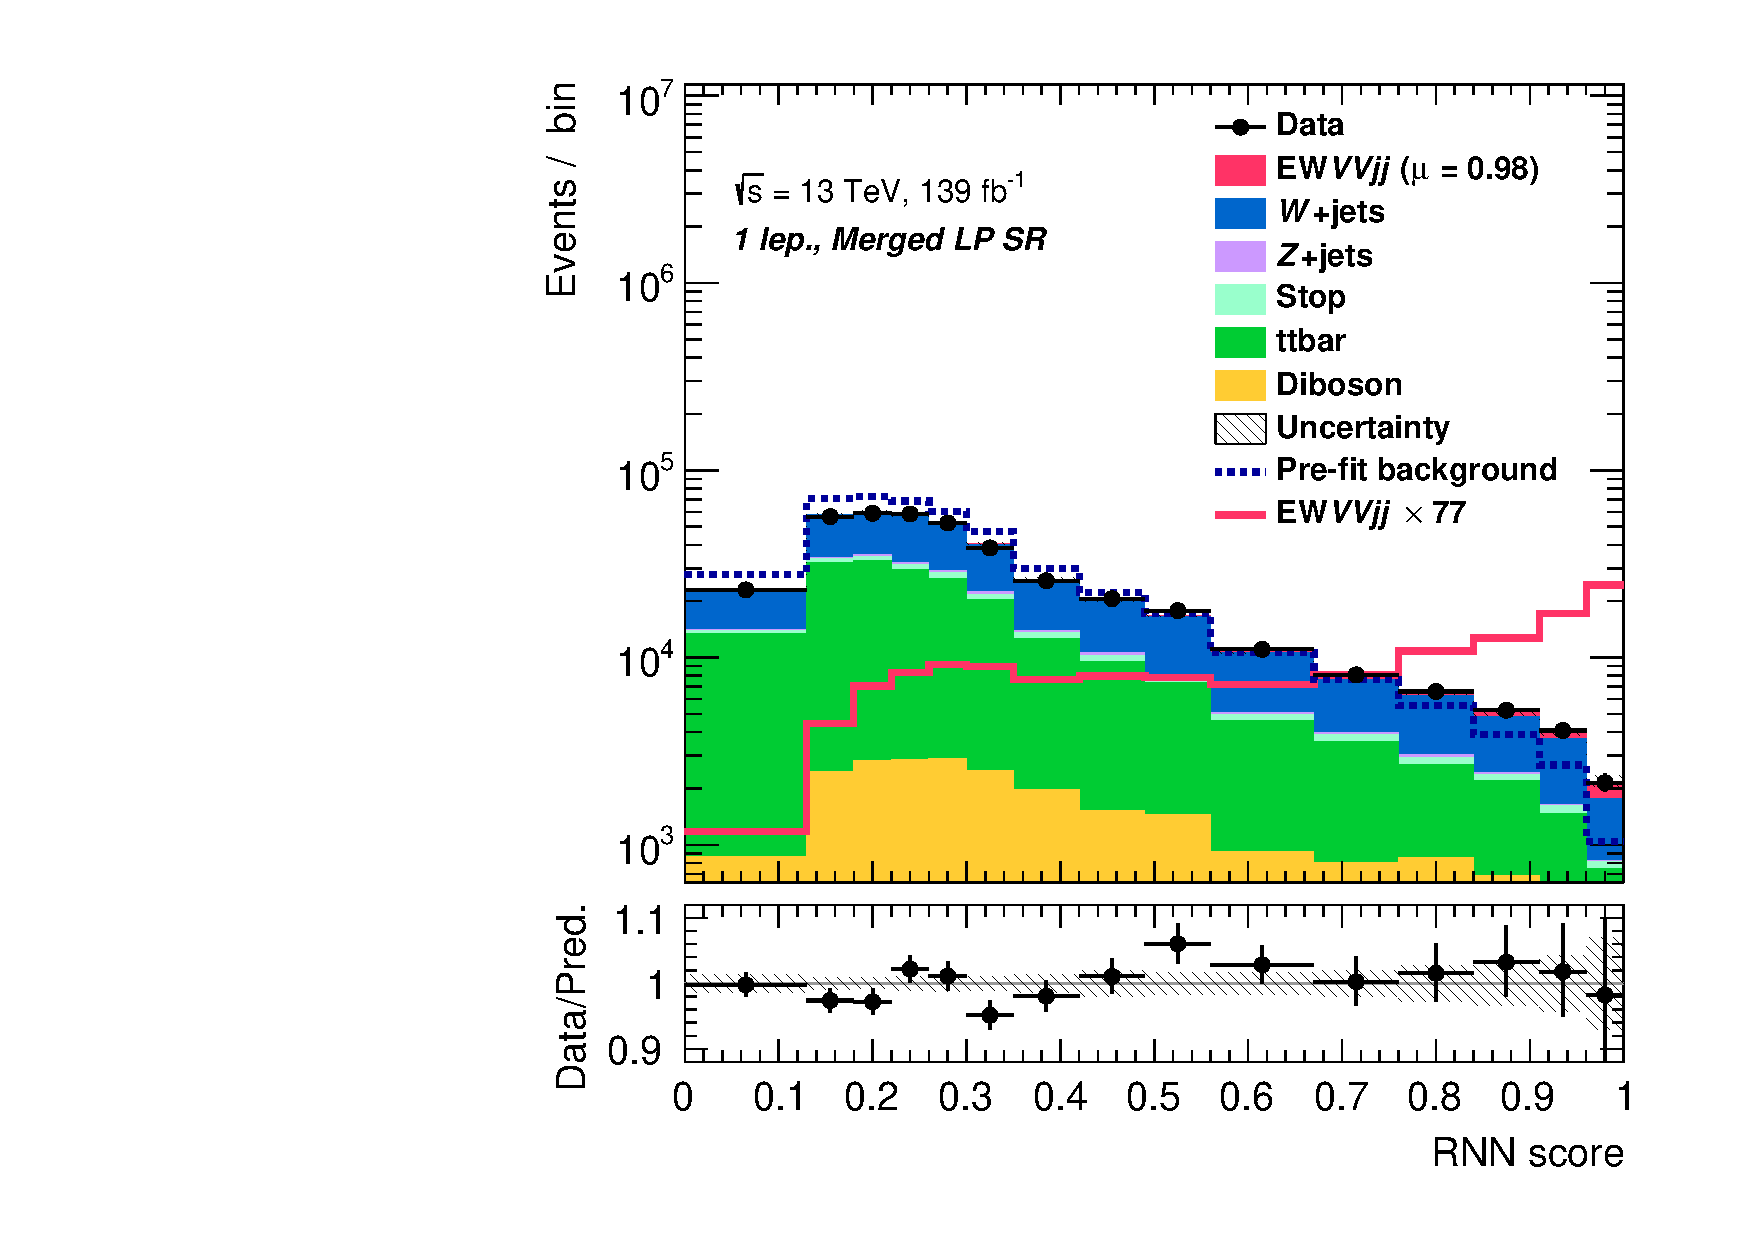
\includegraphics[width=0.45\textwidth]{figures/PostFit/Region_distRNN_DSRVBSLP_BMin0_J0_incJet1_L1_T0_incFat1_Y6051_incTag1_Fat1_GlobalFit_unconditionnal_mu1log}
    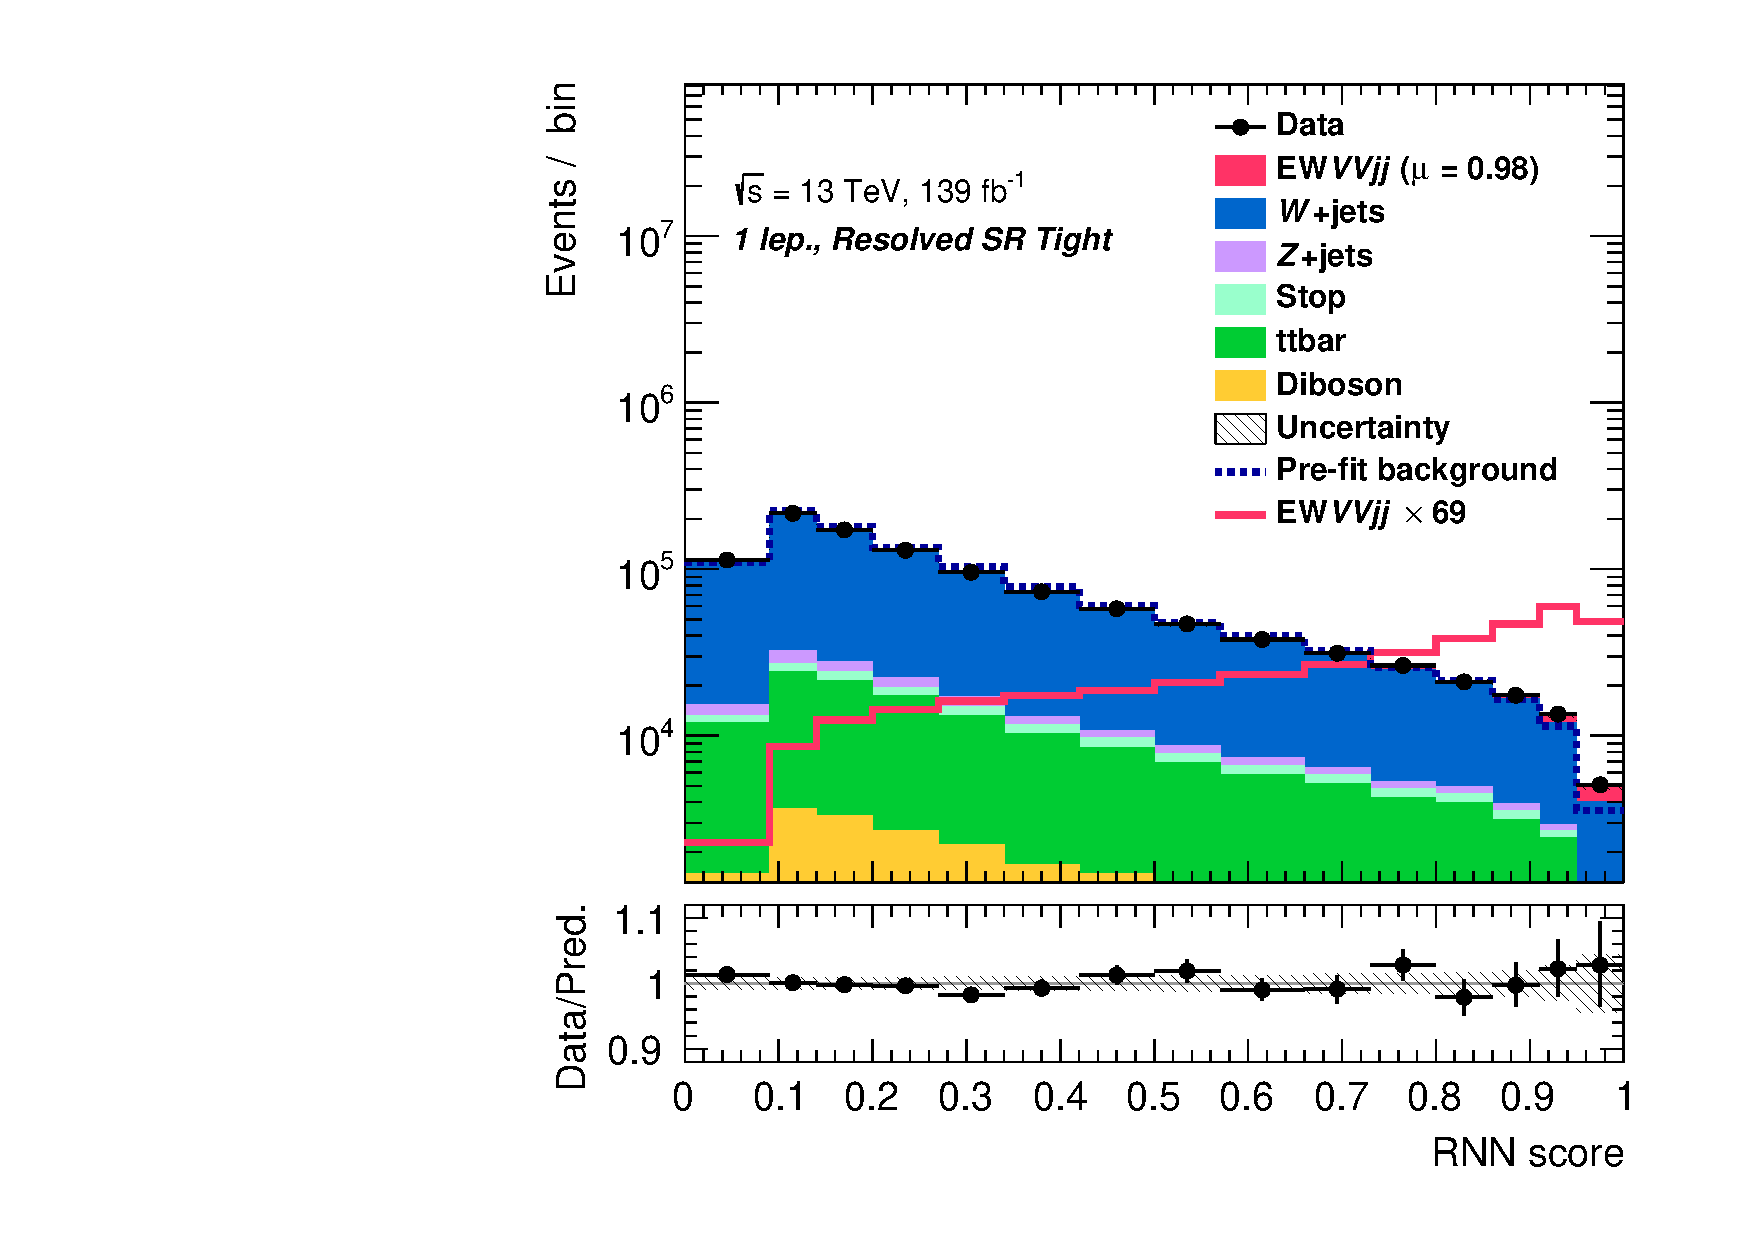
\includegraphics[width=0.45\textwidth]{figures/PostFit/Region_distRNN_DSRVBSTight_BMin0_T0_Y6051_incTag1_J2_L1_incJet1_GlobalFit_unconditionnal_mu1log}
      \caption{Comparisons of the observed data and expected background distributions of RNN score in 1-lepton channel signal regions. The EW VV+jj signal is filled on top of the fitted backgrounds, normalized to the signal yield extracted from the observed data ($\mu = 0.98$). The bottom panel shows the ratio of the observed data to the post fit signal and background predictions.}
      \label{fig:postSR1lep}
\end{figure}
\begin{figure}[]
    \centering
    %2lep
    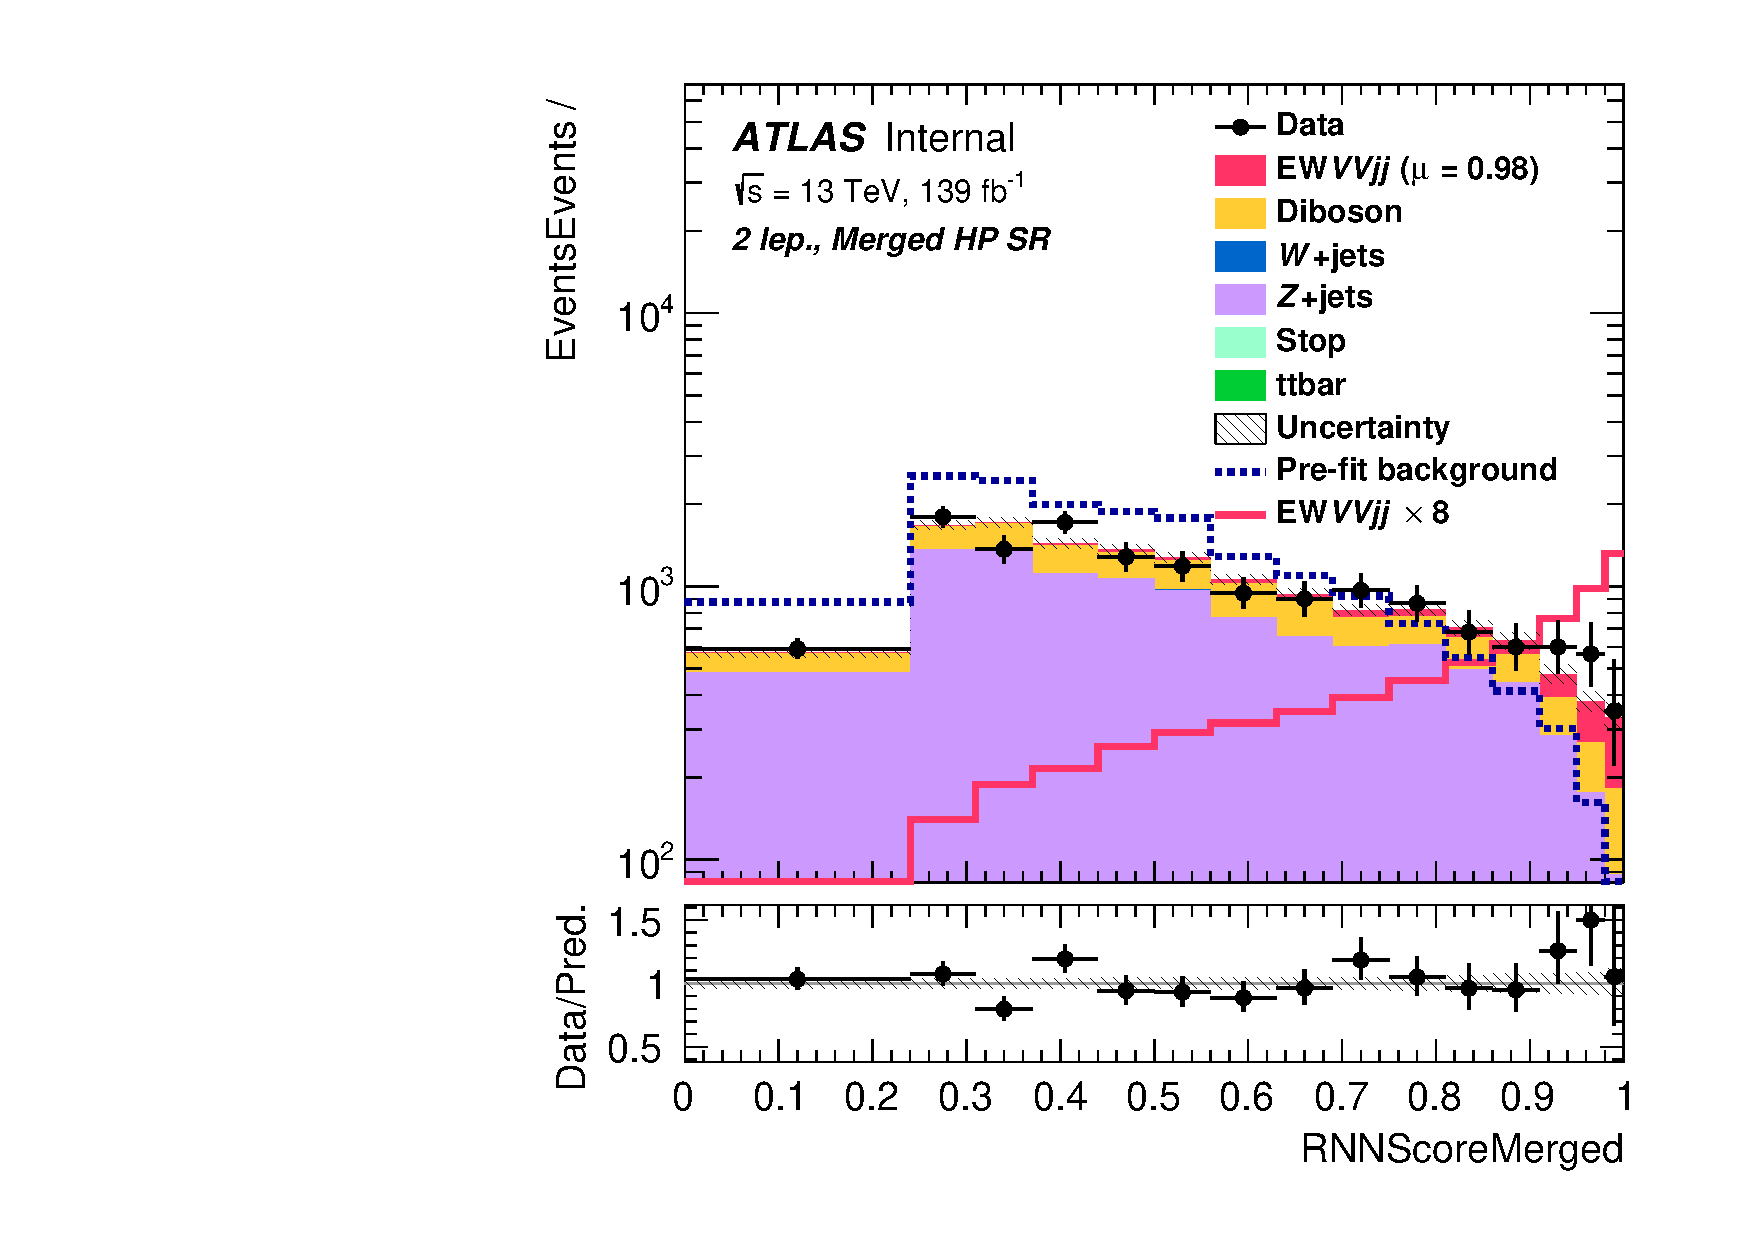
\includegraphics[width=0.45\textwidth]{figures/PostFit/Region_distRNNScoreMerged_DSRVBSHP_BMin0_J0_incJet1_L2_T0_incFat1_Y6051_incTag1_Fat1_GlobalFit_unconditionnal_mu1log}
    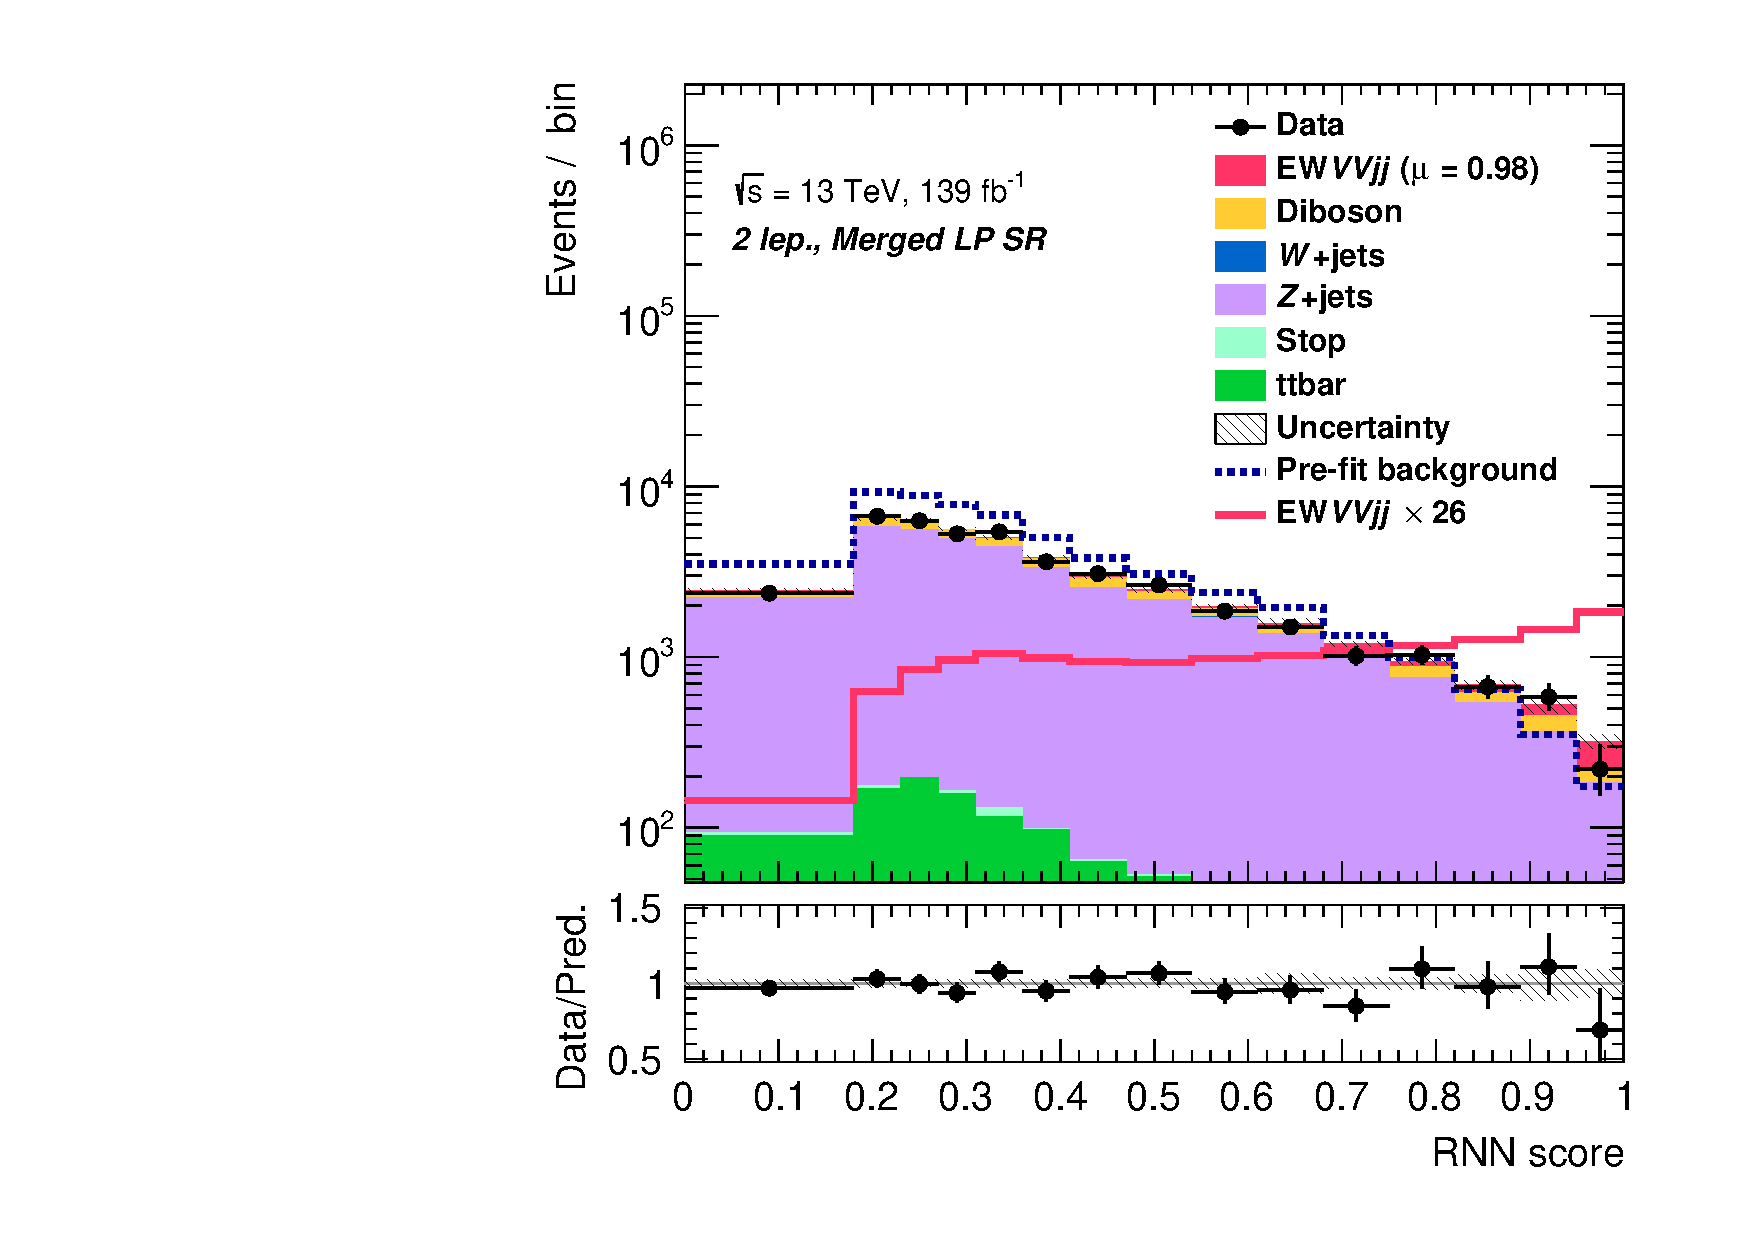
\includegraphics[width=0.45\textwidth]{figures/PostFit/Region_distRNNScoreMerged_DSRVBSLP_BMin0_J0_incJet1_L2_T0_incFat1_Y6051_incTag1_Fat1_GlobalFit_unconditionnal_mu1log}
    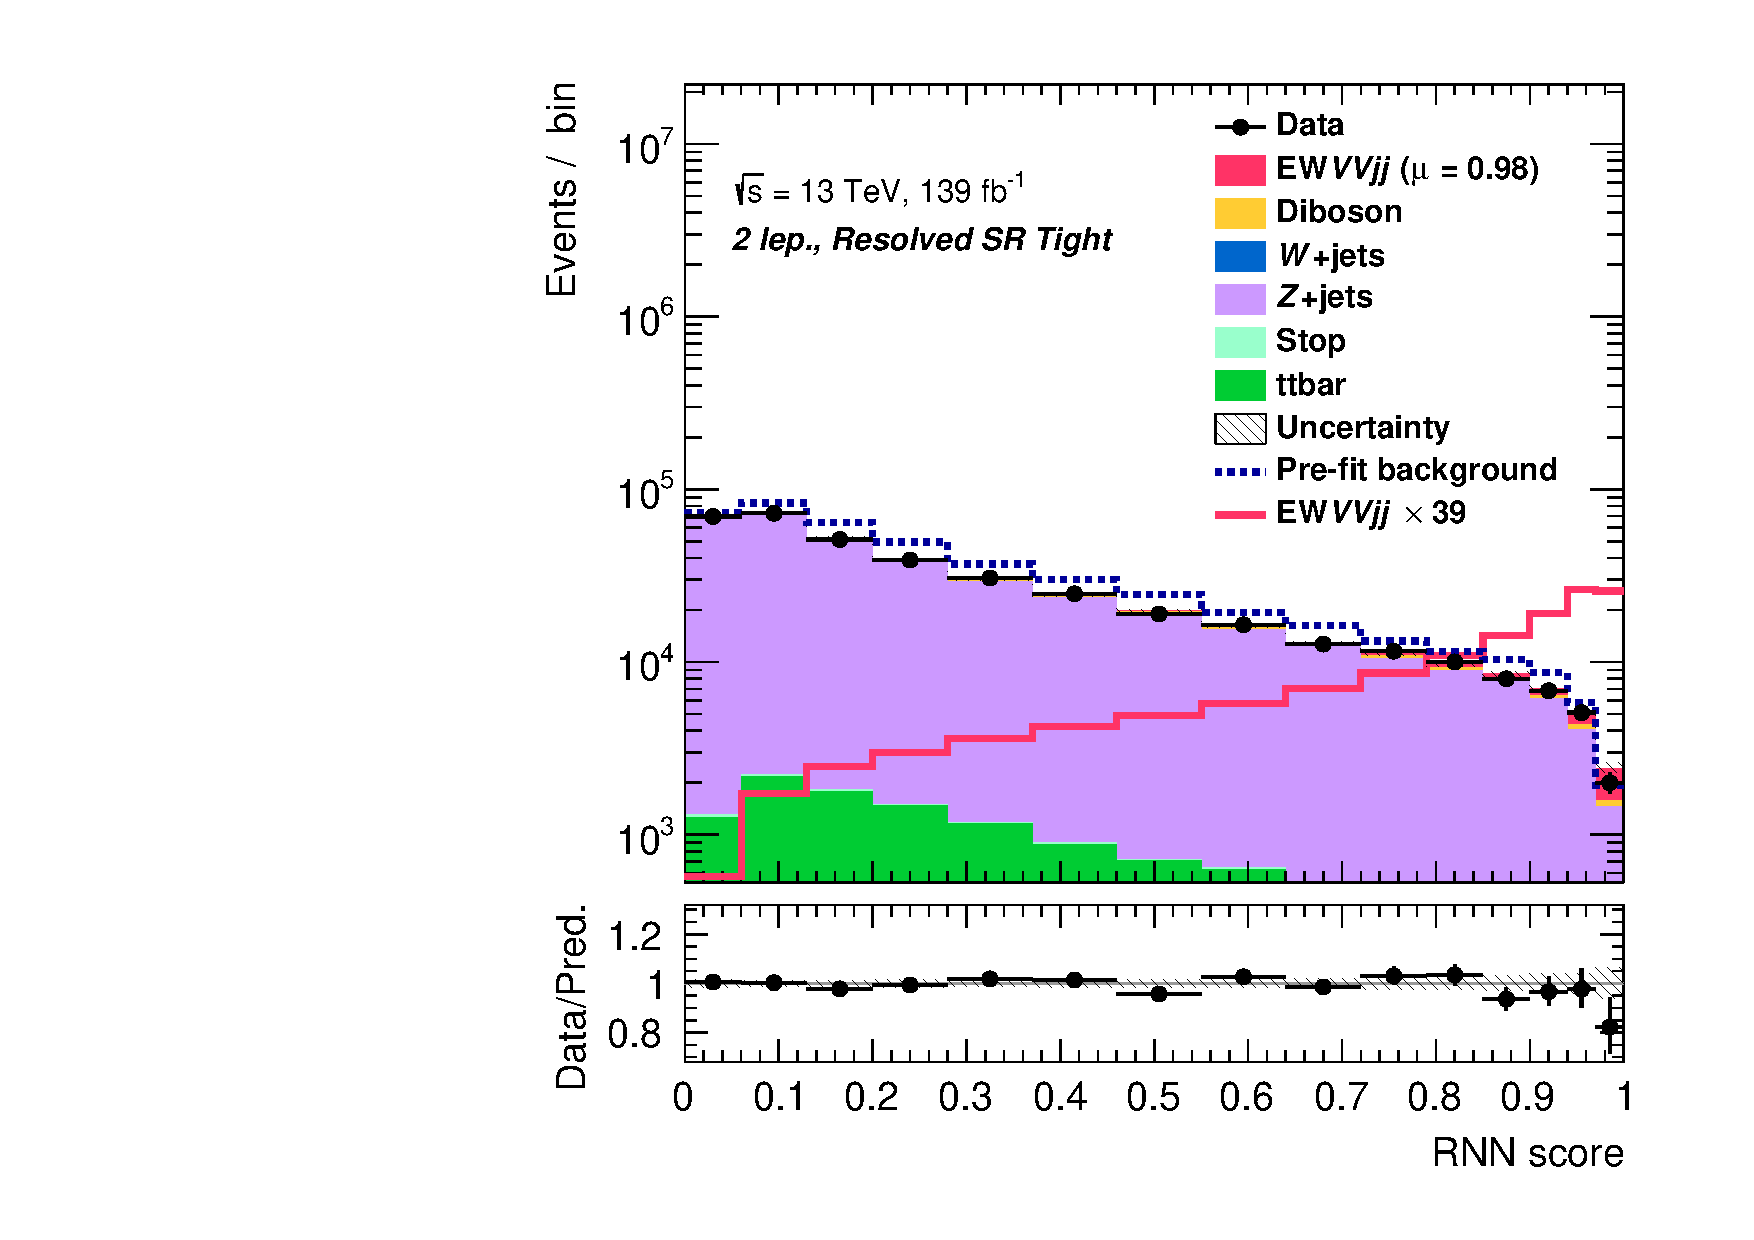
\includegraphics[width=0.45\textwidth]{figures/PostFit/Region_distRNNScoreResolved_DSRVBSFid_BMin0_T0_Y6051_incTag1_J2_L2_incJet1_GlobalFit_unconditionnal_mu1log}
    \caption{Comparisons of the observed data and expected background distributions of RNN score in 2-lepton channel signal regions. The EW VV+jj signal is filled on top of the fitted backgrounds, normalized to the signal yield extracted from the observed data ($\mu = 0.98$). The bottom panel shows the ratio of the observed data to the post fit signal and background predictions.}
    \label{fig:postSR2lep}
\end{figure}


\section{Impact of nuisance parameters on signal strength}
\label{sec:ranking}
%\begin{itemize}
%       \item \texttt{SysTheoryQCD\_Z} 
%        This is the QCD scale uncertainty for the Z+jets background sample. This comes from the %large shape variation in the resolved SR. The input variations are shown in Figure and Figure %in the merged and resolved SRs. \\
%       \item \texttt{MJJREWEIGHT\_100per\_L2\_Fat1} 
%       \item \texttt{MJJREWEIGHT\_100per\_L2\_J2} \\
%       These are the $m^{tag}_{jj}$ reweighting uncertainties for merged and resolved regions. %We expect the large constraints for these uncertainties since these are taken as 100\% %uncertainties.Therefore CRs have large variations and constraints this systematics %uncertainties. \\
%       \item \texttt{SysMODEL\_Z\_MGPy8} \\
%       This is the shape difference between Sherpa Z+jets samples (after the \mjjtag reweighting %applied)and the MadGraph Z+jets samples (no \mjjtag reweighting applied). \\
%       These are expected since there is a well-known large modelling difference between two %generators. \\
%       \item \texttt{SysJET\_Pileup\_OffsetMu} \\
%       This is pile-up related uncertainty.
%       This systematic uncertainty is expected to have a large shape effect on the forward jets.
%%       \\
 %      \item \texttt{SysFATJET\_FatJetTagSF\_Gammajet\_Modelling} \\
 %      This is the uncertainty related to the boosted tagger SF efficiency.
 %      We can see this pull since this uncertainty has a large effect in Merged CR. 
%\end{itemize}

%Some strong pulls (1~$\sigma$ to 1.25~$\sigma$) are observed in the data fit in:
%\begin{itemize}
%    \item \texttt{TheoryQCD\_Z}\\
%    This pull mainly comes from the resolved SRs. Since the impact of this pull is relaxed when %%the left-side bin is merged, this pull seems to comes from the descripance between data to MC i%%%n the RNN left-side bins.
   % \item \texttt{MODEL\_Z\_MGPy8}\\
   % This is coming from the difference in the generators. Since the modeling is better in the %alternative generator, MadGraph, this parameter is pulled a lot to fit to the data.
%\end{itemize}
%The other constraints or pulled (up to 1~$\sigma$) parameters are listed below:
%\begin{itemize}
%    \item \texttt{SysJET\_Pileup\_OffsetMu}\\
%    This is pileup-related uncertainty. This is expected to have a large shape effect on the %forward jet as well as for jet track multiplicity.
%    \item \texttt{SysFATJET\_FatJetTagSF\_Gammajet\_Modeling} \\
%    This is the uncertainty related to the boosted tagger SF efficiency. This pull can be seen %since this  uncertainty has a large effect in Merged CR.
%\end{itemize}

%\subsection{Nuisance Paremeter Correlations}
%The correlation matrix for the Asimov full-range fit for the parameters which has more than 1\% %correlations with any other operators are shown, without statistical uncertainties in each bin %is shown in Figure~\ref{fit_2lep_corr_all}. The strongest correlation of $\minus 78\%$ shows up %%%%between \texttt{MODEL\_Z\_MGPy8} and \texttt{MJJREWEIGHT\_100per\_L2\_J2}. These two par%ameters are both related to the mis-modelling of the Z+jets samples therefore should have cor%relations.
%The parameters which have significant (more than $\pm 30\%$) correlations with the POI %\texttt{$\mu\_$SemileptonicVBS} are:
%\begin{itemize}
%    \item \texttt{TheoryQCD\_Z} 
%    \item \texttt{MODEL\_Z\_MGPy8} \\
%\end{itemize}

%\begin{figure}[ht]
%      \centering
%        \includegraphics[width=\linewidth]%{figures/2lep/FitResults/corr_HighCorrNoMCStat_AsimovAllbins.pdf}%
      %  \caption{Correlations for unconditional fit ($\mu=1$) to asimov data in the full range, for the 2 lepton channel only.}
      % \label{fig:fit_2lep_corr_all}
%\end{figure}

%\section{Rankings}
In order to find out which nuisance parameter impacts the signal strength, the ranking plot for all nuisance parameters is shown in figure~\ref{fig:fit_2lep_ranking_all}. 
The ranking is derived by doing the scans of the likelihood function, by first doing the nominal fit to find the $\hat{\mu}$, then fixing and scanning one NP while all other parameters are fitted again.
%The scan as a function of one parameter stops once the logarithm of the likelihood decreases by 1/2 compared to the global maximum, corresponding to the 1~$\sigma$ uncertainty. 
The change of the signal strength, which is plotted as $\Delta\mu$ is evaluated here.
%The scan is repeated for all NPs, in both direction.

The NP which has the largest impact is the QCD scale systematic uncertainty on EW VV+jj signal sample. 
Varying this QCD scale parameter by $1\sigma$ changes the signal strength by $\Delta \hat{\mu} \simeq \textcolor{blue}{?}$.
The second and third-ranked parameters are for 2-lepton channel, and both are related to the modeling of the Z+jets background sample discussed in chapter~\ref{chap:modeling}.
%The top-two parameters are NPs relates to the Z+jet modeling issue and seen to be pulled in the pull plots. 
%The parameters which have strong impacts and highly-ranked are consistent with the parameters having strong correlations with the POI in the correlation plot, Figure~\ref{fig:fit_2lep_corr_all}.
\begin{figure}[ht]
      \centering
        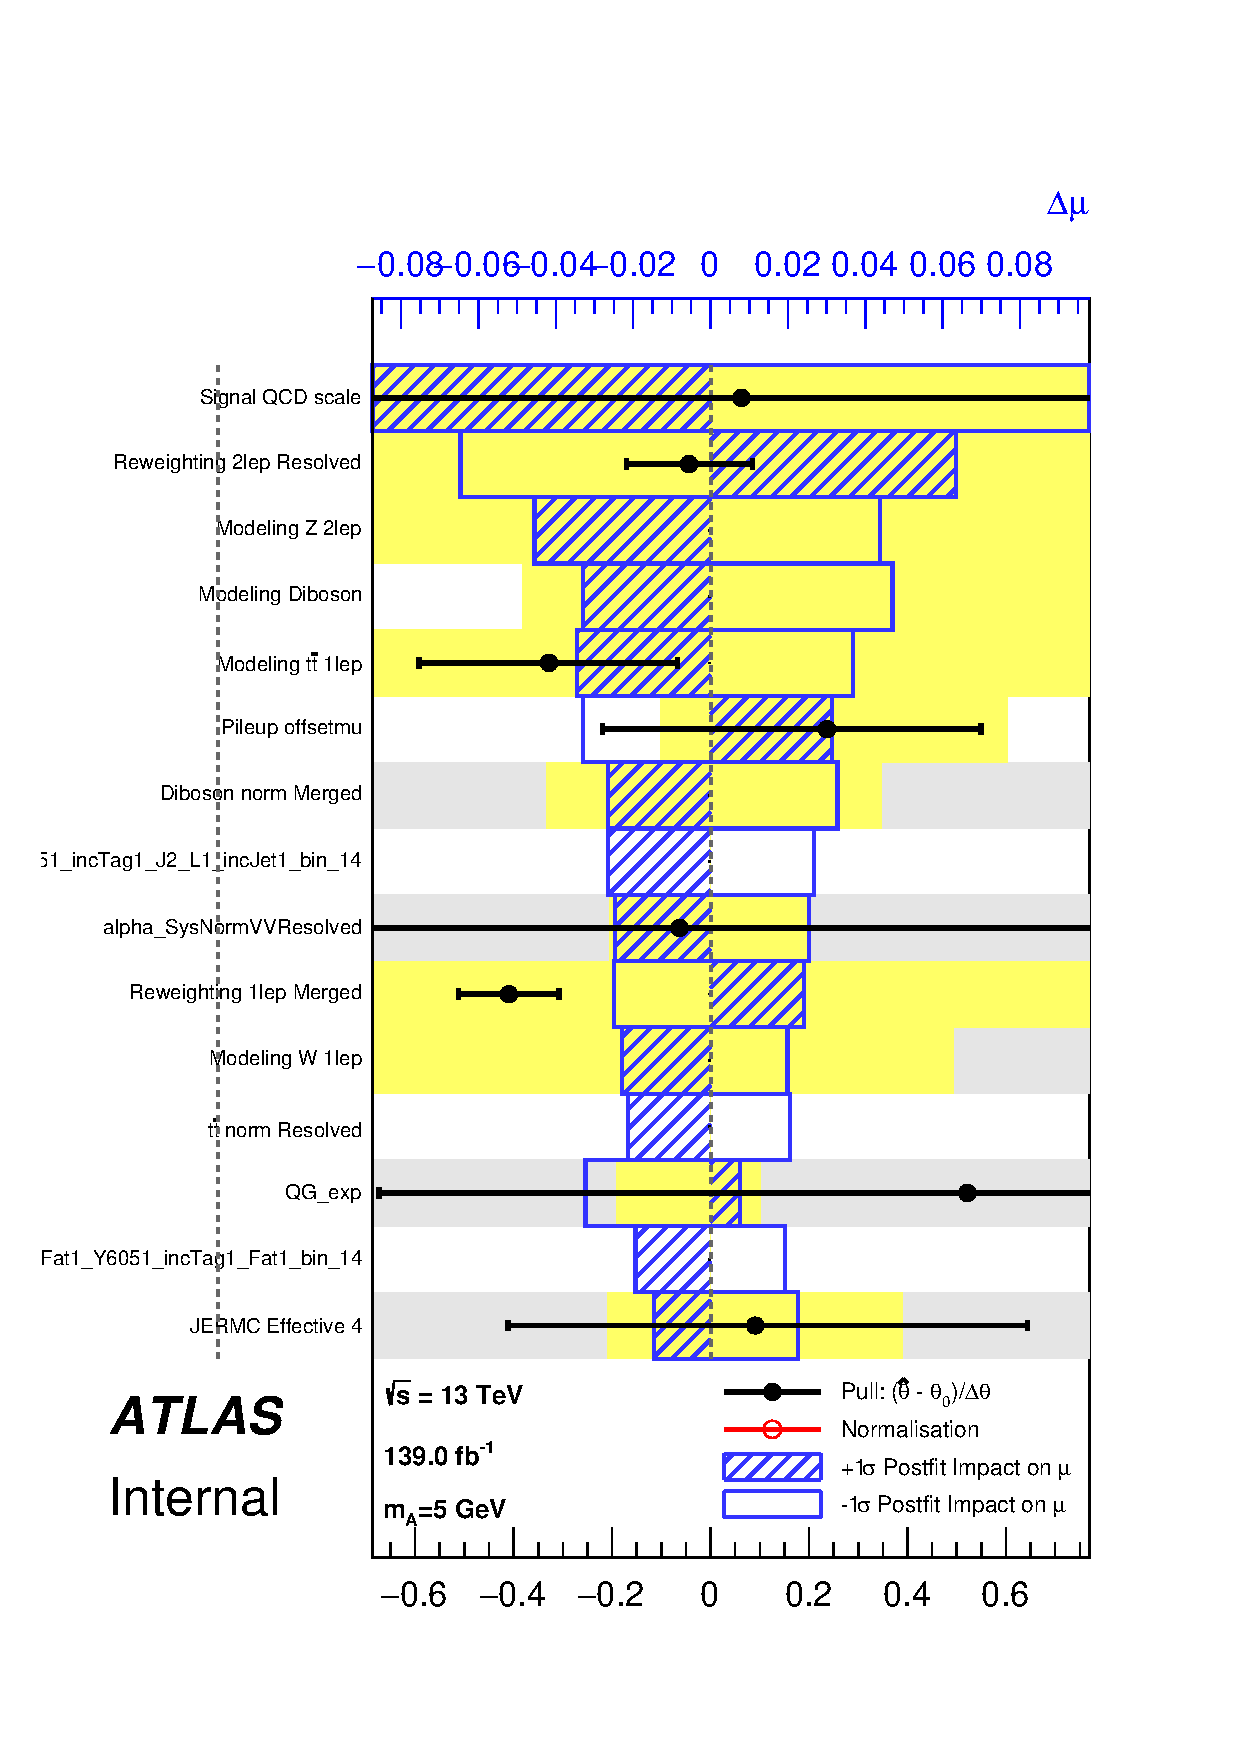
\includegraphics[width=0.60\textwidth]{figures/2lep/FitResults/pulls_mu_SemileptonicVBS_5.pdf}
        \caption{Pre-fit (yellow) and post-fit(blue) nuisance parameter impacts on the signal strength, for all three combined channels. The black and red dots denote pulls ( defined as $(\hat{\theta}-\theta) / \Delta \theta$, where $\Delta \theta$ represents the magnitude of prior uncertainty, and $\theta$ and $\hat{\theta}$ denote pre- and post-fit nuisance parameters) and normalization factors, respectively. \textcolor{blue}{todo: Expand the axis, remove gamma stat}}
       \label{fig:fit_2lep_ranking_all}
\end{figure}

The pulls and constraints for these high-impact parameters are also shown in figure~\ref{fig:fit_2lep_ranking_all} in black dots.
The definition of the pull is $(\hat{\theta}-\theta) / \Delta \theta$, where $\Delta \theta$ represents the magnitude of uncertainty, and $\theta$ and $\hat{\theta}$ denote pre- and post-fit nuisance parameters.
The pull, which can be seen as the deviation of the certain NP from zero, represents how the expectation of that NP does not describe the observed data.
The constraints, which can be seen as the size of the error bar of each uncertainty, represent its reduction from its initial uncertainty value and show how much that uncertainty is constrained by the observed data after fitting.
Ideally the pull and the constraints of certain NP are zero and $1~\sigma$ when the uncertainty is perfectly applied.

The Reweighting systematic uncertainty is highly constrained in figure~\ref{fig:fit_2lep_ranking_all} as designed, same as Modeling Z uncertainty. The Modeling Z uncertainty is pulled about 1~$\sigma$, which seems to be adjusting the Z+jets background to the observed data in the fitting.

All of these highly-ranked NPs are not unexpectedly pulled or constrained, which indicates the likelihood fit performed in this analysis is valid enough.

%The pull plot for all NPs are discussed in Appendix.
%\begin{figure}[ht]
%      \centering
%        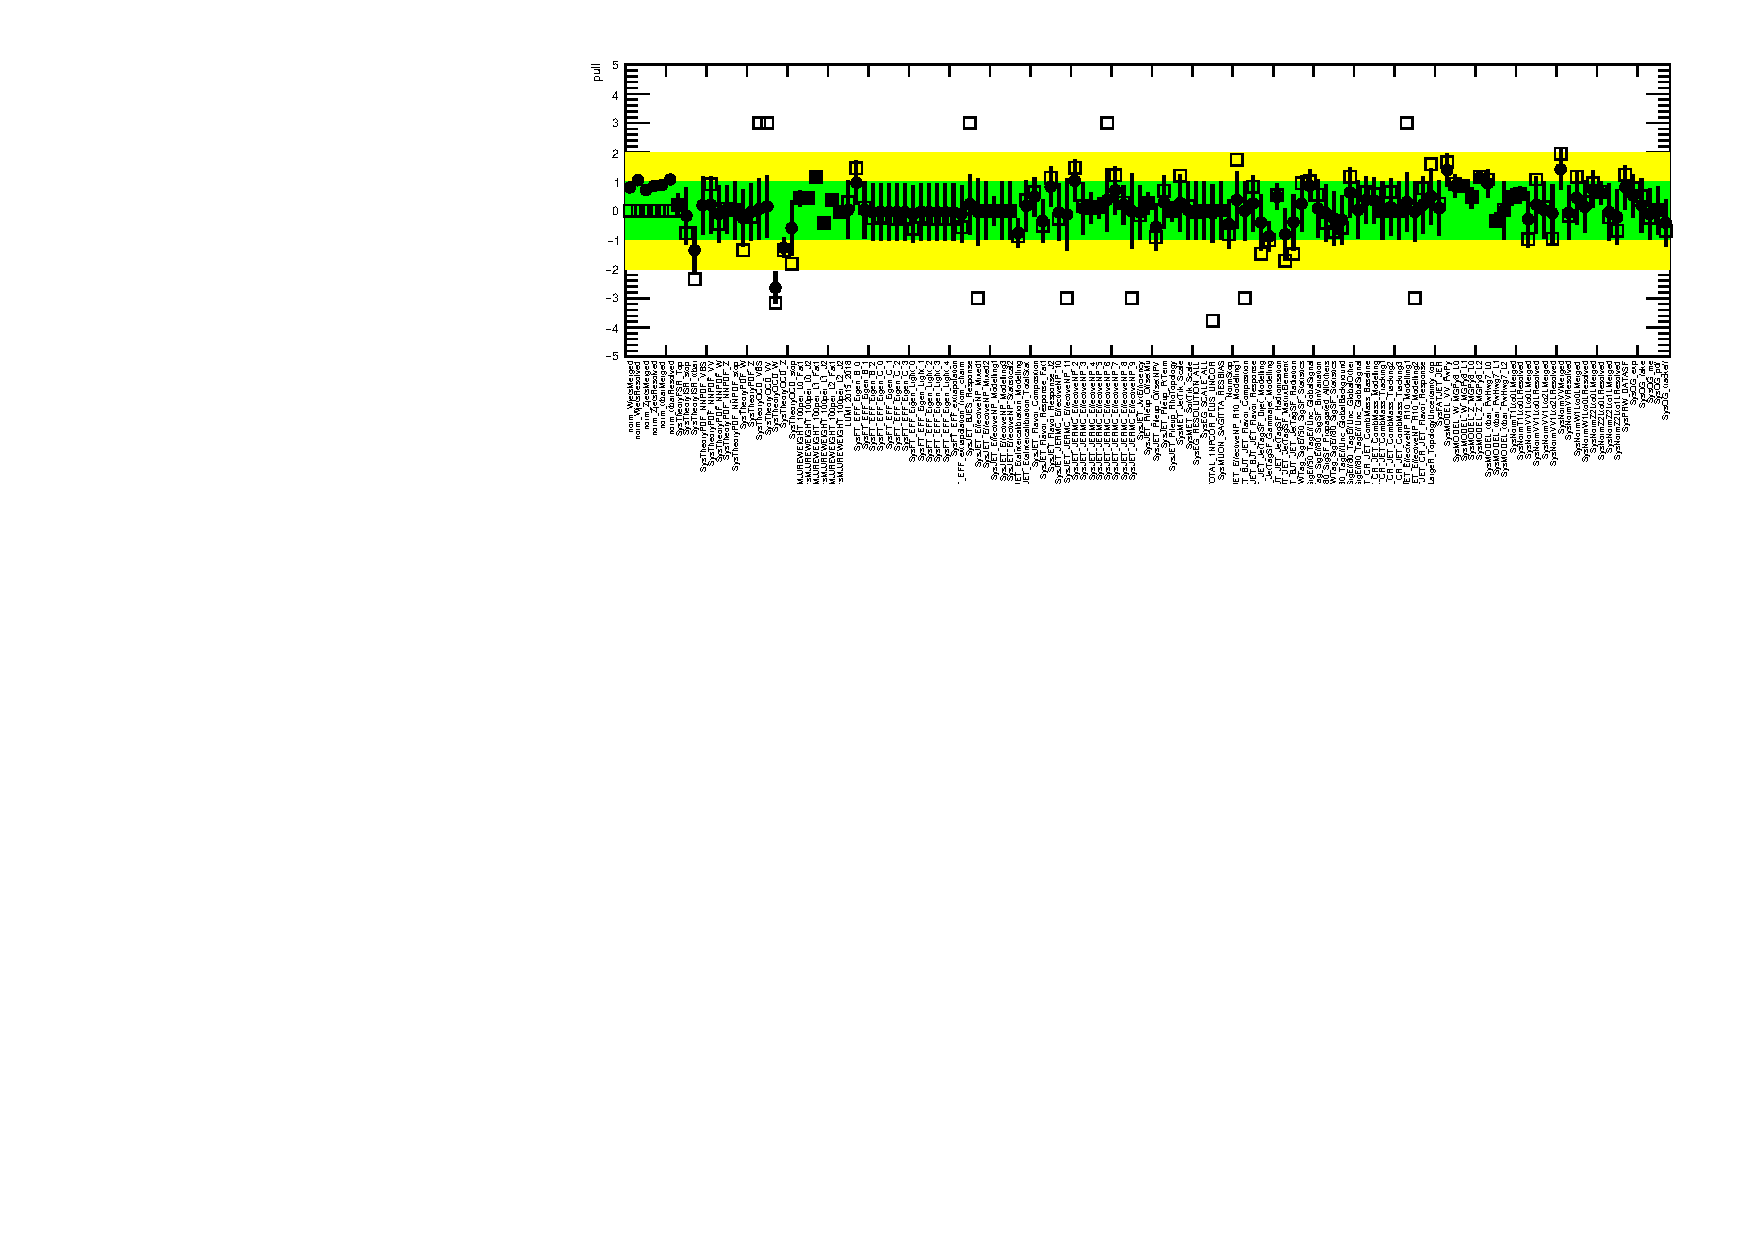
\includegraphics[1.0\textwidth, angle = 270]{figures/2lep/FitResults/NP_allExceptGammas}
%        \caption{\textcolor{blue}{todo: move this pull plot to appendix}}
%       \label{fig:pull}
%\end{figure}

\section{The observed signal strength}
\label{sec:mu}
The estimated signal strength in the fit is:
\begin{equation}
    %\mu = 0.982 \pm 0.217
    \mu = 0.98^{+ 0.22}_{- 0.20} = 0.98^{+ 0.09}_{- 0.09}(\mathrm{Stat})^{+ 0.21}_{- 0.18}(\mathrm{Syst}) 
\end{equation}
The corresponding observed (expected) significance is 5.90 (6.04)~$\sigma$, which claims the observation of the EW VV+jj signal in the semileptonic final state. 
The expected significance is estimated by replacing the nuisance parameter values of the Asimov dataset (an artificial dataset with MC simulations) with those derived from a conditional $\mu = 1$ fit, a fit with $\mu$ fixed at 1, to the data. 

